\documentclass[12pt]{scrartcl} 
\usepackage[left=1in,right=1in,top=1in,bottom=1in]{geometry} 
\usepackage{booktabs}
\usepackage{dcolumn}
\usepackage{setspace}
\usepackage{graphicx}
\usepackage{fullpage}
\usepackage{paralist}
\usepackage{natbib}
\usepackage{appendix}
\usepackage{amsmath}
\usepackage{amsfonts}
\usepackage{amssymb}
\usepackage{color}
\usepackage{times}
\usepackage{topcapt}
\usepackage{booktabs}
\usepackage{rotating}
\usepackage{sectsty}
\usepackage{morefloats}
\usepackage{url}
\sectionfont{\large}
\subsectionfont{\normalsize}
\subsubsectionfont{\small}

\title{\Large{An Analysis of Racially Polarized Voting in Arizona}}
\author{Gary King \thanks{king@harvard.edu} 
\and 
Benjamin Schneer \thanks{bschneer@fas.harvard.edu}
}

\date{January 25, 2011}

\begin{document}
\maketitle

\doublespacing

\section{Introduction}

We have been retained by the Independent Arizona Redistricting
Commission to analyze data from the maps drawn for the 2011-2012
redistricting cycle. In this report, we estimate the extent of
racially polarized voting in Arizona, determine the electability of
the minority groups' candidates of choice, and (through a new method
new method we introduced for this purpose) evaluated whether stronger
districts could have been drawn.  We perform this analysis for both
the benchmark map and proposed map, which allows for a judgment of
whether the proposed map has a retrogressive effect.

% A summary of our findings is as follows:

% \begin{itemize}
% \item Finding One
% \item Finding Two
% \item Finding Three
% \end{itemize}

\subsection{Methodological Approach}

To analyze the maps under consideration, we must provide evidence
about the voting behavior of different ethnic groups. However, direct
evidence is unavailable because of the secret ballot. Thus, methods of
ecological inference are used to estimate (rather than determineq)
individual voting behavior based upon VTD-level aggregated election
results as well as VTD-level voting age population from the US Census.

In 1953, two methods of ecological inference were introduced -- the
method of bounds \citep{duncan1953} and ecological regression
\citep{goodman1953}. A special case of the method of bounds is known
as �homogeneous precinct analysis,� which had been used in many court
cases: this approach seeks out ethnically homogeneous precincts (100\%
black, 100\% white, or 100\% Hispanic) because for those precincts we
know for certain the voting behavior of an ethnic group. The
assumption behind this method is that the voting behavior observed in
homogeneous precincts is identical to that in other areas. The
advantage of this method is that it yields completely certain
information about some subgroups of voters; the disadvantage is that
the relatively few who live in homogeneous precincts may turnout in
different numbers and vote for different candidates in starkly
different ways than the vast majority of the population who live in at
least partially heterogeneous areas.

The second method of ecological inference -- ecological regression --
ignores the information revealed by the method of bounds and its
special case of homogeneous precinct analysis. Instead, ecological
regressions gather hints from statistical information across all
precincts. For example, if we find that in areas with more African
Americans that more votes are cast for the Democrats, then we may
infer that it is the African Americans who are voting for the
Democrats. The advantage of this approach is that it uses some
information from all precincts. The disadvantage is that the
information can be highly misleading: For example, also consistent
with the evidence would be that the whites who live in areas with many
African Americans are the ones who are producing more votes for the
Democrats. In fact, as an indication of the substantial problems with
this method, ecological regression, unlike the method of bounds,
regularly gives impossible answers -- such as the percent of Hispanics
voting for the Democrats of 160\% or -54\%.

The method of bounds (or homogeneous precinct analysis) and ecological regression dominated the academic literature and courtroom expert testimony from 1953 until 1997 when \citeauthor{king1997}'s EI approach was introduced. King's approach was the first to combine the deterministic information from the method of bounds with the statistical information from ecological regression into a single set of estimates. Thus, it uses the statistical information from all precincts, the certain information from homogeneous precincts, and other deterministic information known for certain from other precincts. Impossible estimates are never produced by this methodology, and all information from all precincts are used in the analysis. Like any indirect method of revealing information that the secret ballot hides, EI is also uncertain to a degree, but it uses more information than any other approach. Since 1997, a variety of other methods have been developed in the academic literature by King and others, virtually all of which now follow King's practice of including deterministic and statistical information in the same model. For example, \citet{king2001} extends King's method to arbitrarily large numbers of ethnic groups and candidates; we use this method in our work as well as King's original method. Some of these other methods have been collected in the edited volume by \citet{king2004}.

In practice, when we have data we can use to validate the methods, ecological regression and homogeneous precinct analysis tend to be fairly inaccurate most of the time. Studies have shown that uncertainty remains with King's and subsequent methods, but the estimates are normally superior. Differences among the methods that do include both deterministic and statistical information are, in comparison, relatively minor.

In this case, we use these newer methods to give estimates of the proportion of each ethnic group that votes and, among those voting, that votes for each of the candidates. We also use King's �tomography plots� and other diagnostic methods that help us discern when adjustments in the methods need to be made.
And finally, we have used the results from the ecological inference analysis to measure what we call district performance, which is the percent of the voting age population which a given ethnic group needs in order to receive a specified share of the vote -- in this case we use 50 or 55 percent as the specified thresholds. We do this under the assumption that voters in a racial group in the district will have the same voting behavior as voters in a racial group from adjacent districts.

\subsection{Elections Analyzed}
We have examined elections in the state of Arizona from 2004 through 2010. These elections include: 2004 US Presidential Election, 2006 Arizona Secretary of State Election, 2008 US Presidential Election, 2010 Arizona Mine Inspector Election and 2010 Arizona Secretary of State Election. All of these are state or national elections and therefore are considered ``exogenous'' elections in the sense that changes in district lines should not influence the vote choice of individual voters. Minority candidates ran for office in four of these five elections. Specifically, Hispanic candidates served as the Democratic candidate in the 2006 Arizona Secretary of State Election and 2010 Arizona Mine Inspector Election; an African-American candidate served as the Democratic candidate in the 2008 US Presidential Election; a Native American was the Democratic candidate in the 2010 Secretary of State Election. The 2004 US Presidential Election did not include a minority candidate; however, as we show below, the Democratic Presidential candidate appears to be the clear candidate of choice for minority voters in most districts.

\section{Analysis of Congressional Districts}

We have used ecological inference in order to determine the extent of racially polarized voting in Arizona as well as the electability of each district's candidate of choice among minority voters. For each congressional district in the benchmark and proposed map, we estimated the turnout and vote shares for each minority group. To illustrate our approach, we describe the analysis for the vote totals for a single election occurring in a single congressional district.

Table~\ref{smine_cvap_cd_3_ex} displays estimates of how each racial group in the proposed Congressional District 3 voted in the 2010 election for Arizona Mine Inspector. Note that in each table the row and column totals are {\it observed} while the internal cells are {\it estimated}. The bottom row labeled Total Pop gives the total population vote totals computed by aggregating over all VTDs in the district. Similarly, the column labeled Total CVAP lists the share of citizen voting age population comprised by each racial group in the district. Again, this is calculated by simply aggregating over all VTDs in the district. 

\begin{table}[ht]
\begin{center}
\caption{Mine Inspector 2010 CD 3 (Proposed)}
\label{smine_cvap_cd_3_ex}
\begin{tabular}{lccccc}
  \hline
Racial Group & Turnout & D Vote & R Vote & S Vote & Total CVAP\\ 
  \hline
White & 0.36 & 0.35 & 0.65 & 0.00 & 0.43 \\ 
  Hispanic & 0.30 & 0.90 & 0.10 & 0.00 & 0.44 \\ 
  Native American & 0.22 & 0.90 & 0.09 & 0.01 & 0.04 \\ 
  Black & 0.13 & 0.50 & 0.48 & 0.02 & 0.05 \\ 
  Other & 0.21 & 0.55 & 0.44 & 0.01 & 0.05 \\ 
  Total Pop & 0.31 & 0.61 & 0.39 & 0.00 &  \\ 
   \hline
\end{tabular}
\end{center}
\end{table}

The internal cells in the table contain the estimates from ecological inference. For example, we estimate that Hispanic citizens in CD 3 voted for the Democratic Candidate at a rate of 90\% and for the Republican candidate at a rate of 10\%, and 0\% for any third party candidates. Furthermore, Hispanics made up 44\% of the districts total population (CVAP) and turned out for the election at a rate of 30\%. Looking at the district as a whole, the Democratic candidate received 61\% of the vote. Thus, for the 2010 Mine Inspector election in the proposed CD 3, the Democratic candidate was the clear candidate of choice for Hispanic voters and this candidate comfortably carried the district despite the existence of some level of polarized voting (i.e., lower support among white voters who we estimate voted for the Democrat at a rate of 35\%). 

This example illustrates the method of analysis for a single race in a single district. We conducted this form of analysis for each district in each election of interest.\footnote{The results presented here use the Citizen Voting Age Population (CVAP) totals. We present the same set of estimates using Voting Age Population (VAP) totals in the digital appendix.} In the sections that follow, we use our estimates for each district and election to assess the level of racial polarization and ability to elect the candidate of choice.

We have included tables illustrating the estimates for each district and each race in the appendix of this report.

\subsection{Sources of Uncertainty}
There are several sources of uncertainty in these estimates including estimation uncertainty, fundamental uncertainty, and model dependence. Estimation uncertainty occurs because we have a limited set of observations to use in estimating how each racial group votes. Fundamental uncertainty is the idea that even with a large amount of data there is some degree of randomness in the electoral process. We address this by simulating each election 50,000 times in order to determine estimates that reflect the most likely outcome. Finally, model dependence occurs because the underlying assumptions of the model almost never exactly reflect the exact empirical process that is being studied. In the estimation performed for this report, model dependence serves as the most significant source of uncertainty that we must take into account. 

To convey the degree of uncertainty in the estimates of turnout and vote share, we use tomography plots to accompany the tables \citep{king1997}.  These plots give all information in the data without making any statistical modeling assumptions, as well as summarizing the available statistical information in the data. One plot is needed for each estimate in the corresponding table. For example, the tomography plot below analyzes the information and uncertainty in the data and our analyses with respect to the percent of Whites (horizontally) and non-Whites (vertically) who vote for the Hispanic candidate in District 3, in each precinct. If this information were known for a precinct, it would appear in the plot as a single dot, and the set of precincts as a set of dots. Because of the secret ballot, we cannot know the exact point with precision; what the plot shows is that the information hidden from us by the secret ballot is directly quantifiable: it turns each precinct's dot into a line.  We can think of the dot as being smeared into a line. That smearing represents a loss of information, but much information is retained (and that is uniquely captured by  our methods of ecological inference).

\begin{figure}[htb]
\begin{centering}
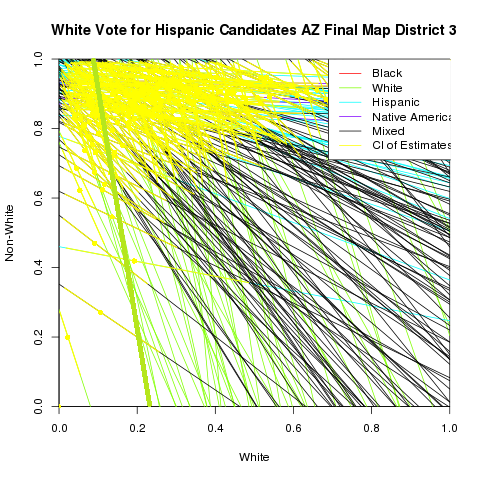
\includegraphics[scale=.5]{pl_whitevote_h_3.png}
\caption{This tomography plot displays the white vote for the Hispanic Candidate in 2010 Mine Inspector Election}
\end{centering}
\label{tomog}
\end{figure}

For example, consider the bold green line in the plot. We know, based on the observed data, that the point in this plot (representing where the White and non-White vote share is) for this precinct must be some point on the line, but we do not know exactly where on the line this point falls. For this line, we know that the fraction of Whites that vote for the Hispanic candidate must fall somewhere between 0.16 (16 percent) and 0.23 (23 percent). We get these numbers by projecting the line downwards to the horizontal axis. If instead we project the line to the left (vertical) axis, we can see that, for this particular precinct, the range of possible values for the percent of non-Whites voting for the Hispanic candidate could be anywhere from 0\% to 100\%. That estimate is better than the method of ecological regression, which often gives answers outside that interval, but still we can see that this precinct is informative with respect only to Whites, not non-Whites. In this way, each line captures exactly what we do and do not know about the voting behavior in each precinct. Our statistical method uses all this available information. Lines that are relatively steep in this particular tomography plot, convey a lot of information about the percent of Whites that vote for the Hispanic candidate. Lines that are relatively flat convey a great deal of information about the percent of non-Whites voting for the Hispanic candidate. Lines that cut off the top right or bottom left corner of the plot are informative about both quantities.

The tomography plots reflect what we know about the racial composition of each precinct. If a precinct contains more than 65\% of a particular racial group (which we use as an arbitrary cutoff for graphical clarity), then the line on the tomography plot that corresponds to that precinct is color coded to represent the majority group (see the legend in the plot). If no groups comprise 65\% or more of the precinct, then no color code is assigned. 
Finally, the tomography plots also reflect the results of the ecological inference statistical estimation. The point estimate (i.e., the exact point on the line that we estimate as the vote share for each group) as well as the confidence intervals are colored yellow. Taken together, these describe the overall estimate of how racial groups voted in the district as a whole. For example, in the tomography plot for District 3 we estimate that white voters voted for the Hispanic candidate at a substantially lower rate than did their non-white counterparts in the district.  
The point of the tomography plots is to convey the overall uncertainty and certainty in the available data, and how our statistical estimator uses that information to produce an estimate. The uncertainty estimates here are far more informative and information rich than sampling based confidence intervals or standard errors.

For the sake of conciseness, tomography plots for each estimate are included in a digital appendix.

\subsection{Racially Polarized Voting}
We assess the degree of racially polarized voting in both the benchmark and proposed districts using Tables~\ref{smine_cvap_cd_3} through~\ref{sos10_cvap_cd_7_benchmark} in the appendix, which displays the estimates for proposed CDs 3 and 7 as well as benchmark CDs 4 and 7. 

The proposed CDs 3 and 7 both demonstrate a high degree of polarized voting between whites and the ``main minority'' Hispanics. For both districts, the clear candidate of choice for the main minority across all five elections is the Democratic candidate; however, white voters do not appear to prefer the main minority candidate of choice. For example, as Table~\ref{smine_cvap_cd_7} illustrates, 90\% of Hispanic voters in CD 7 preferred the Democratic candidate in the 2010 Arizona Mine Inspector while there was an even split among white voters for this candidate. A similar trend holds across all other elections for both CD 3 and CD 7 in the proposed map.

\begin{figure}[!h]
\begin{centering}
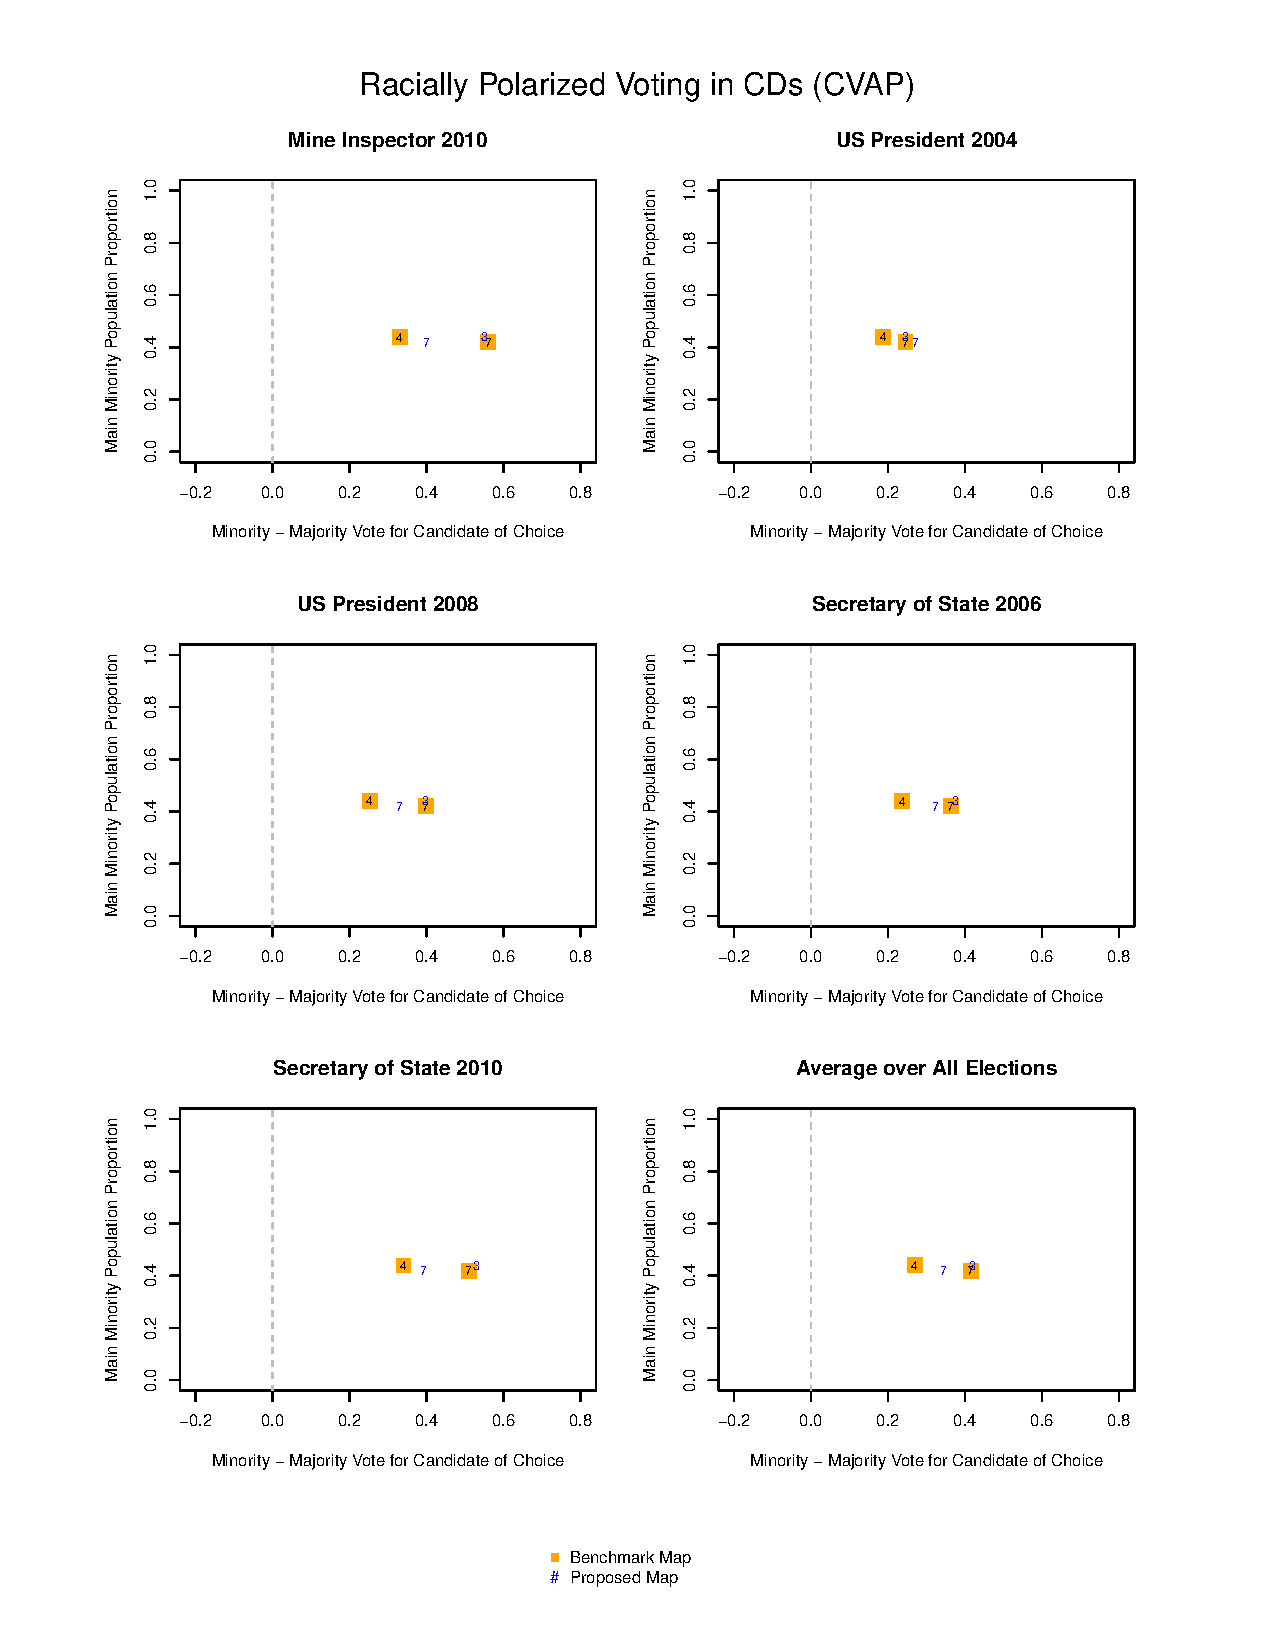
\includegraphics[scale=.8]{cvap_cd_polarization.pdf}
\caption{CVAP Congressional Districts: Racial Polarized Voting}
\end{centering}
\label{cvap_cd_polarization}
\end{figure}

The benchmark map's congressional districts reveal a similar level of polarization. For example, as Table~\ref{smine_cvap_cd_7_benchmark} illustrates, 89\% of Hispanic voters favored the Democratic candidate in the benchmark CD 7 while only 33\% of whites voters voted for the minority candidate of choice.

Figure~\ref{cvap_cd_polarization} displays the level of racially polarized voting across all races and also provides an easy graphical means of comparing racial polarization between the proposed and benchmark districts.

In each graph, the horizontal axis represents the main minority (Hispanic) vote minus the majority (white) vote for each district. Thus, districts located farther to the right exhibit higher levels of polarized voting. The vertical axis tracks the share of the main minority (Hispanic) population in each district. The orange squares represent the location of the benchmark districts while the blue numbers represent the proposed districts.

As is evident from figure~\ref{cvap_cd_polarization}, the level of polarization from benchmark to proposed is strikingly similar across all races. Proposed CD 3 exhibits a level of polarization almost identical to benchmark CD 7. Proposed CD 7 exhibits a slight but insubstantial level of polarization over the benchmark CD 4. Furthermore, the proposed districts maintain a similar level of main minority population as compared to the benchmark.

\subsection{Electability of Candidate of Choice}
We assess the electability of the candidate of choice in both the benchmark and proposed districts using Tables~\ref{smine_cvap_cd_3} through~\ref{sos10_cvap_cd_7_benchmark} in the appendix, which displays the estimates for proposed congressional districts 3 and 7 as well as benchmark congressional districts 4 and 7.

Figure~\ref{cvap_cd} displays the results of our analysis; this figure is particularly crucial because it helps provide answers to the questions that are at the heart of whether the proposed districts are retrogressive or not. In particular, for each election the figure captures (1) the {\it estimated} level of support  among the main minority group in each congressional district candidate for the candidate of choice; (2) the {\it observed} electability of the candidate of choice in each congressional district; and, (3) the degree to which the proposed districts represent improvement or retrogression along these two dimensions.

\begin{figure}[!h]
\begin{centering}
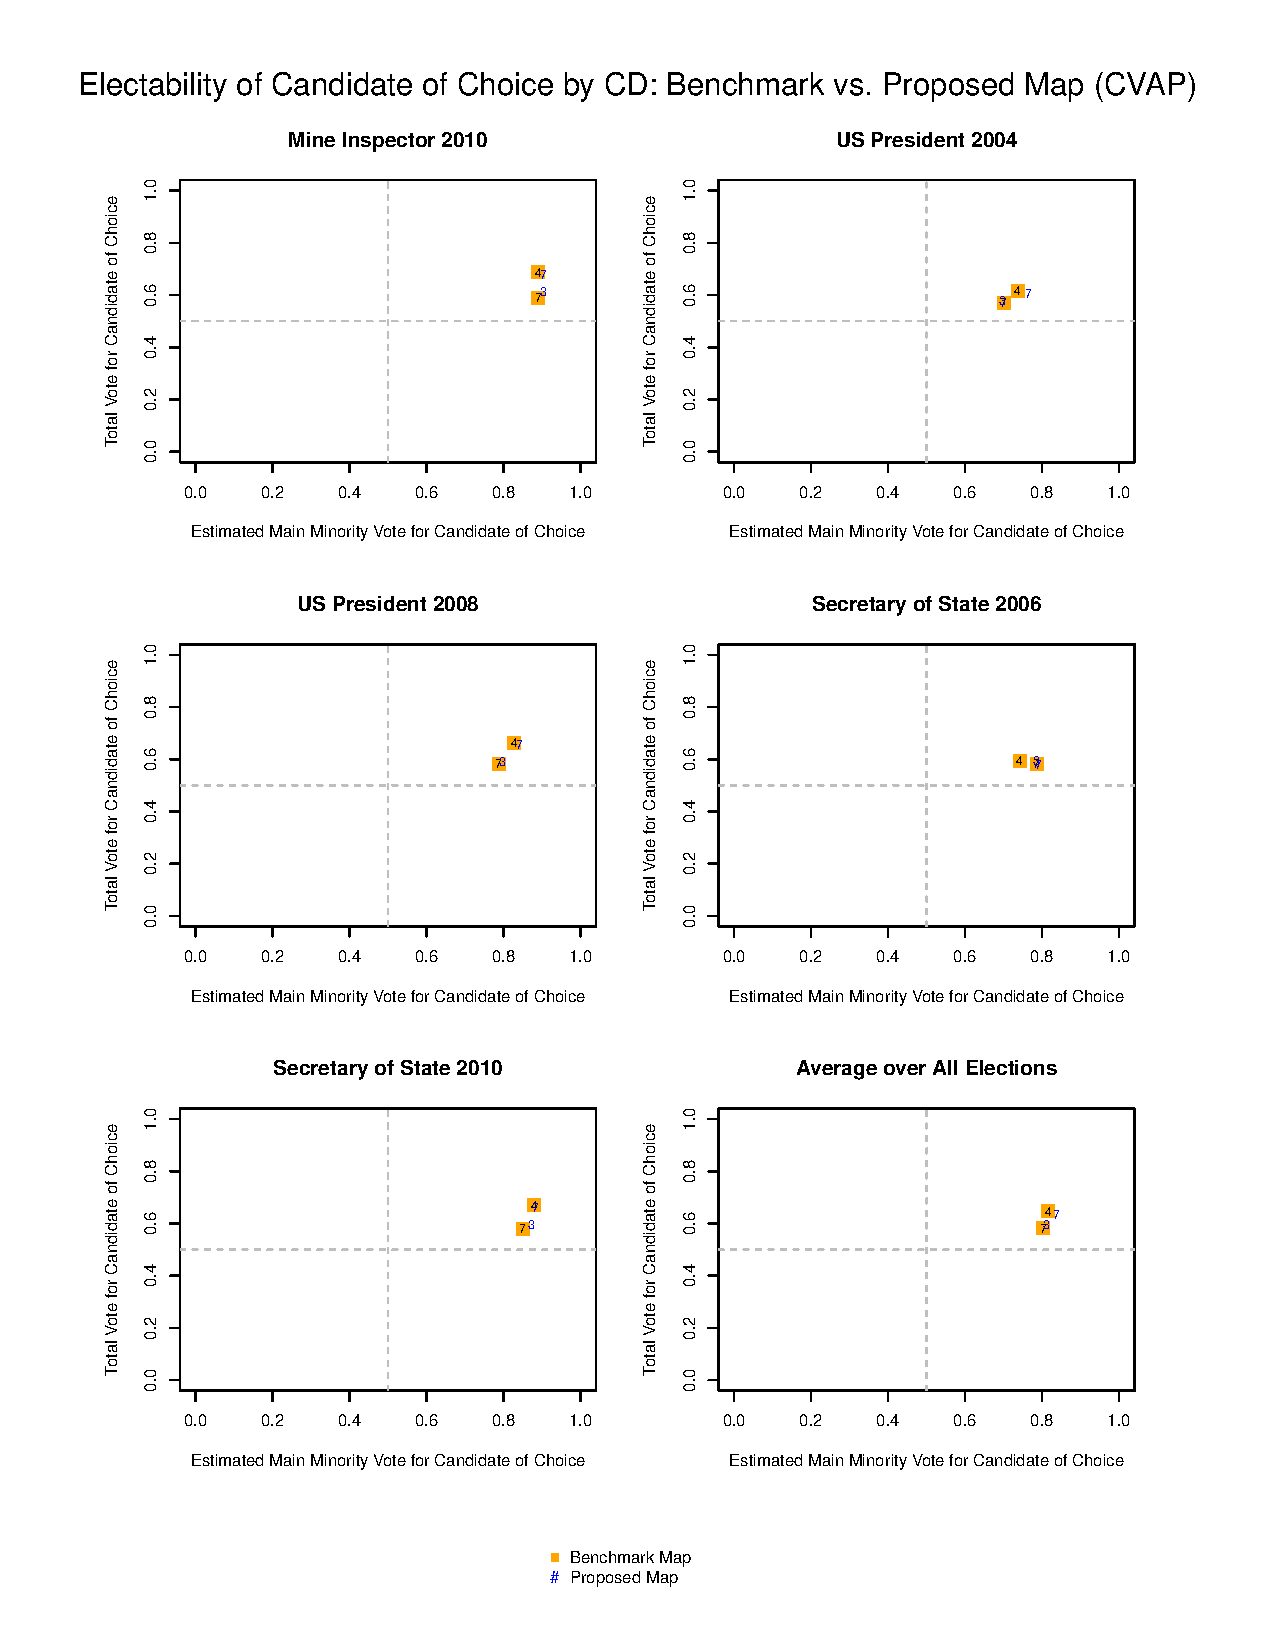
\includegraphics[scale=.8]{cvap_cd.pdf}
\caption{CVAP Congressional Districts}
\end{centering}
\label{cvap_cd}
\end{figure}

For each graph in figure~\ref{cvap_cd}, the horizontal axis captures the estimated two-party vote share for the candidate of choice among the main minority population. The vertical axis represents the observed two-party vote share for the candidate of choice in the district. Thus, when a district falls in the top right quadrant of a graph it means that that (1) the main minority in the district prefers the candidate of choice and (2) the district as a whole would have elected the candidate of choice. 

As the figure illustrates, across all five individual elections (and when averaging across the five elections as in the graph in the bottom right corner) proposed CDs 3 and 7 fall in the top right quadrant -- these districts demonstrate a clear candidate of choice and maintain the ability to elect that candidate. 

Furthermore, the graphs reveal that for each election the proposed districts perform as well or better than the benchmark districts in terms of both the existence of a clear main minority candidate of choice as well as the ability to elect this candidate. Based on these criteria, the proposed districts do not appear to be retrogressive when compared to the benchmark districts.

%\subsection{The Potential for Stronger Districts: A Counterfactual Analysis}

%\begin{figure}[htb!]
%\begin{centering}
%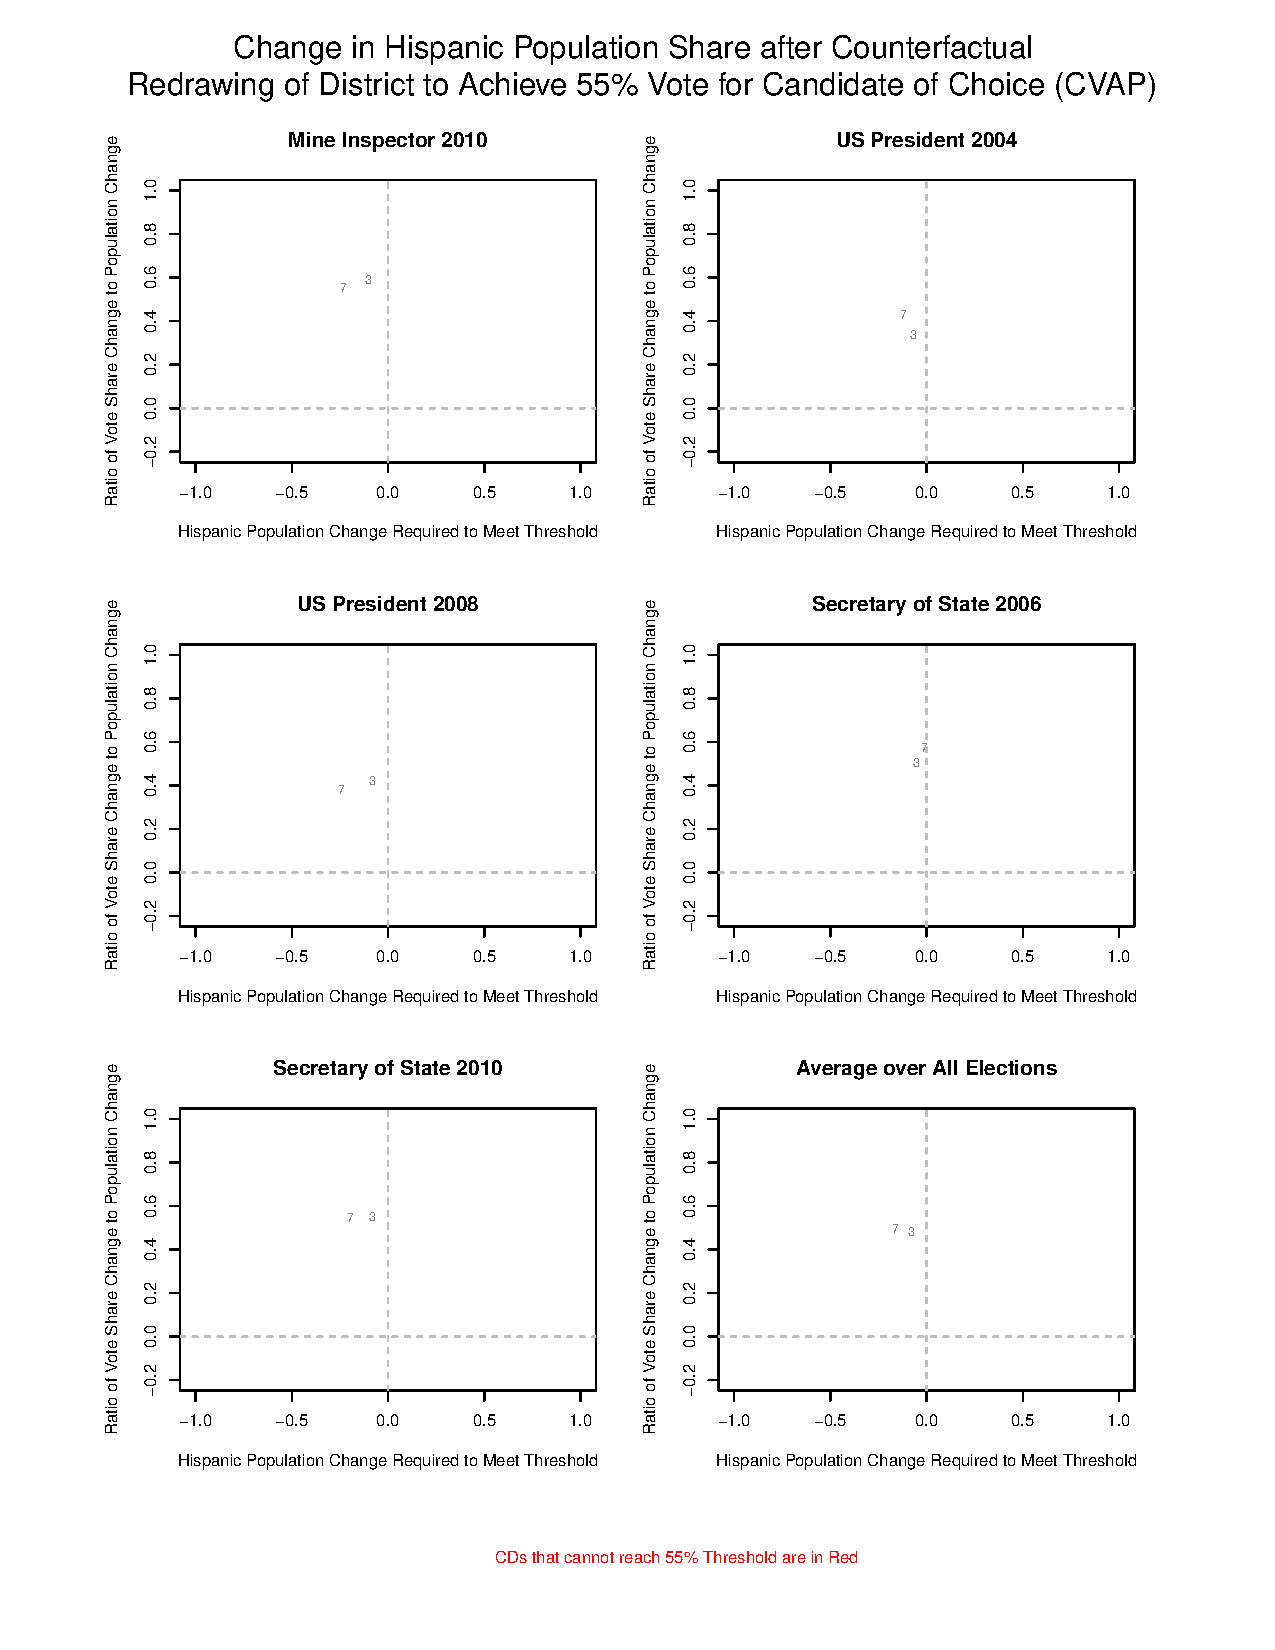
\includegraphics[scale=.8]{cvap_cd_performance_ratio.pdf}
%\caption{CVAP Congressional Districts}
%\end{centering}
%\label{cvap_cd_performance_ratio}
%\end{figure}

\section{Analysis of Legislative Districts}

\subsection{Racially Polarized Voting}

\begin{figure}[ht]
\begin{centering}
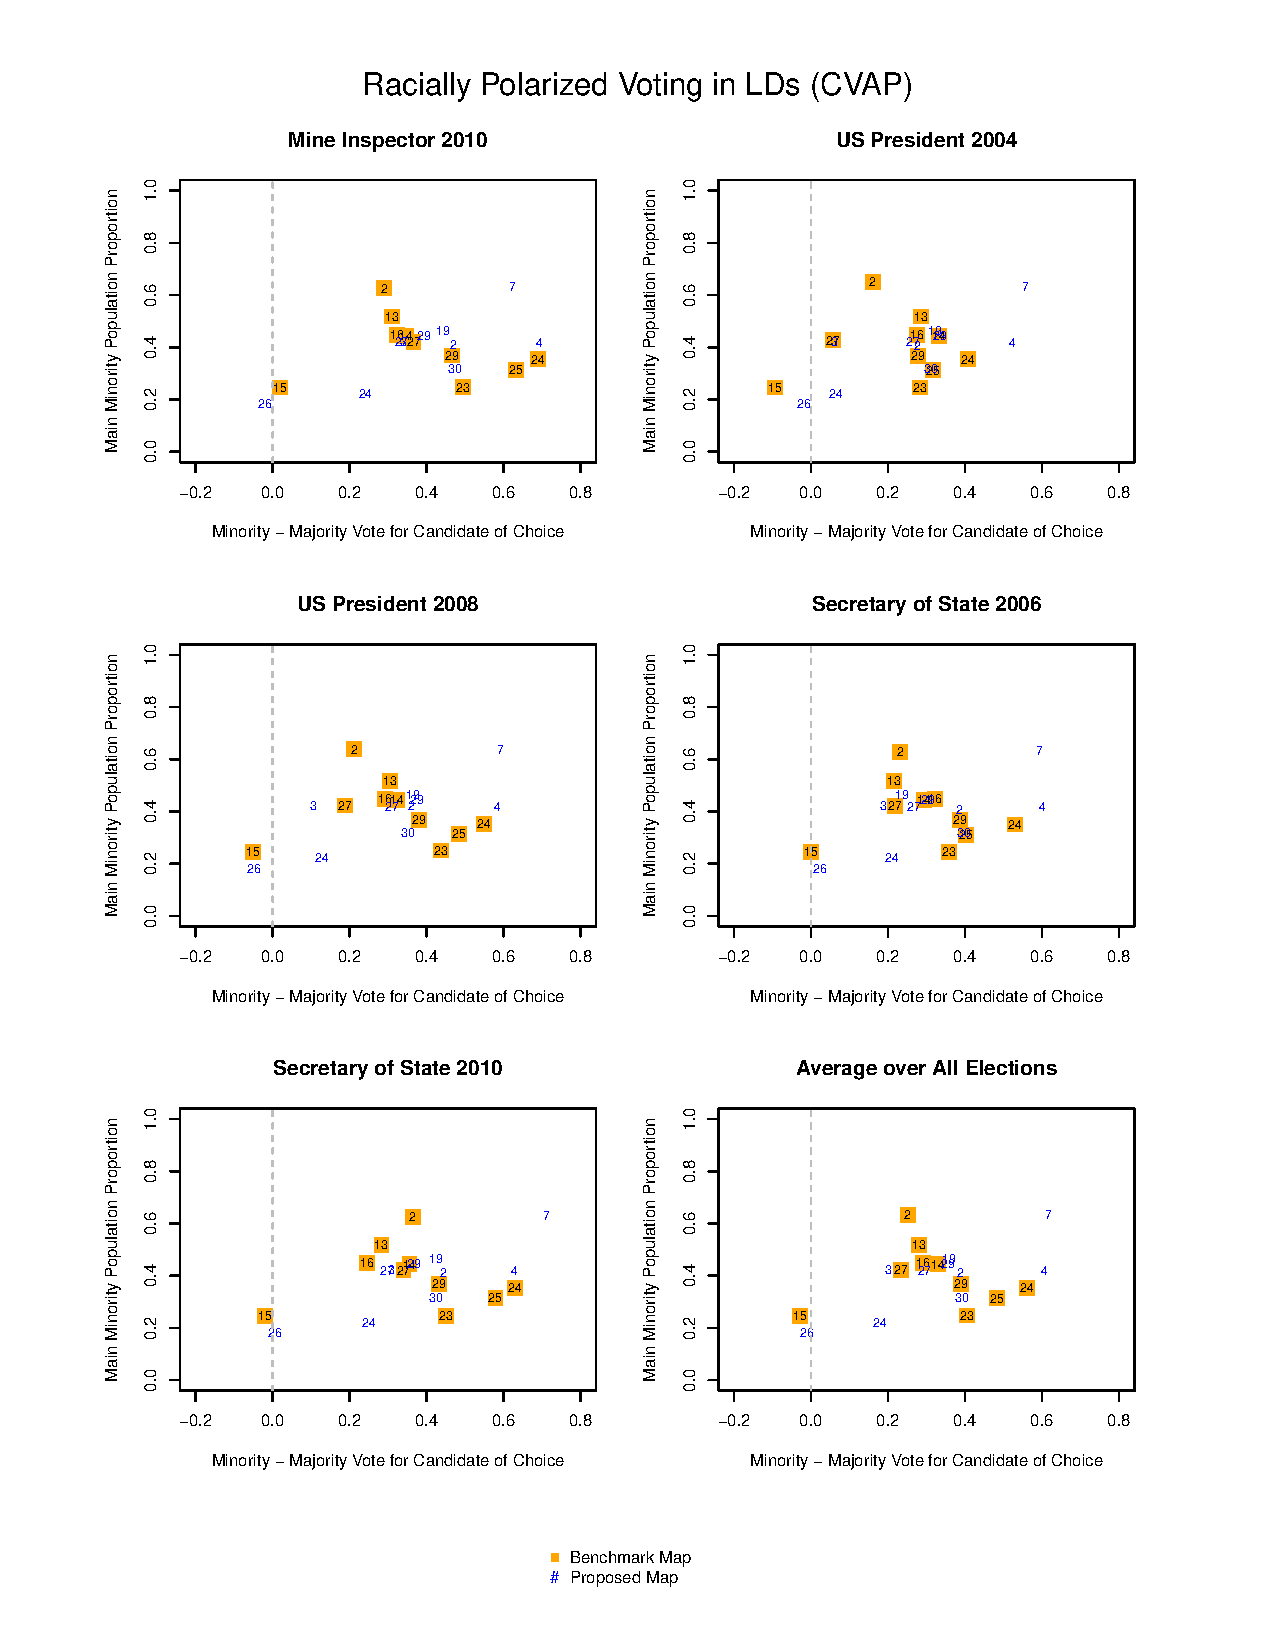
\includegraphics[scale=.8]{cvap_ld_polarization.pdf}
\caption{CVAP Legislative Districts}
\end{centering}
\end{figure}

\subsection{Electability of Candidate of Choice}

\begin{figure}[ht]
\begin{centering}
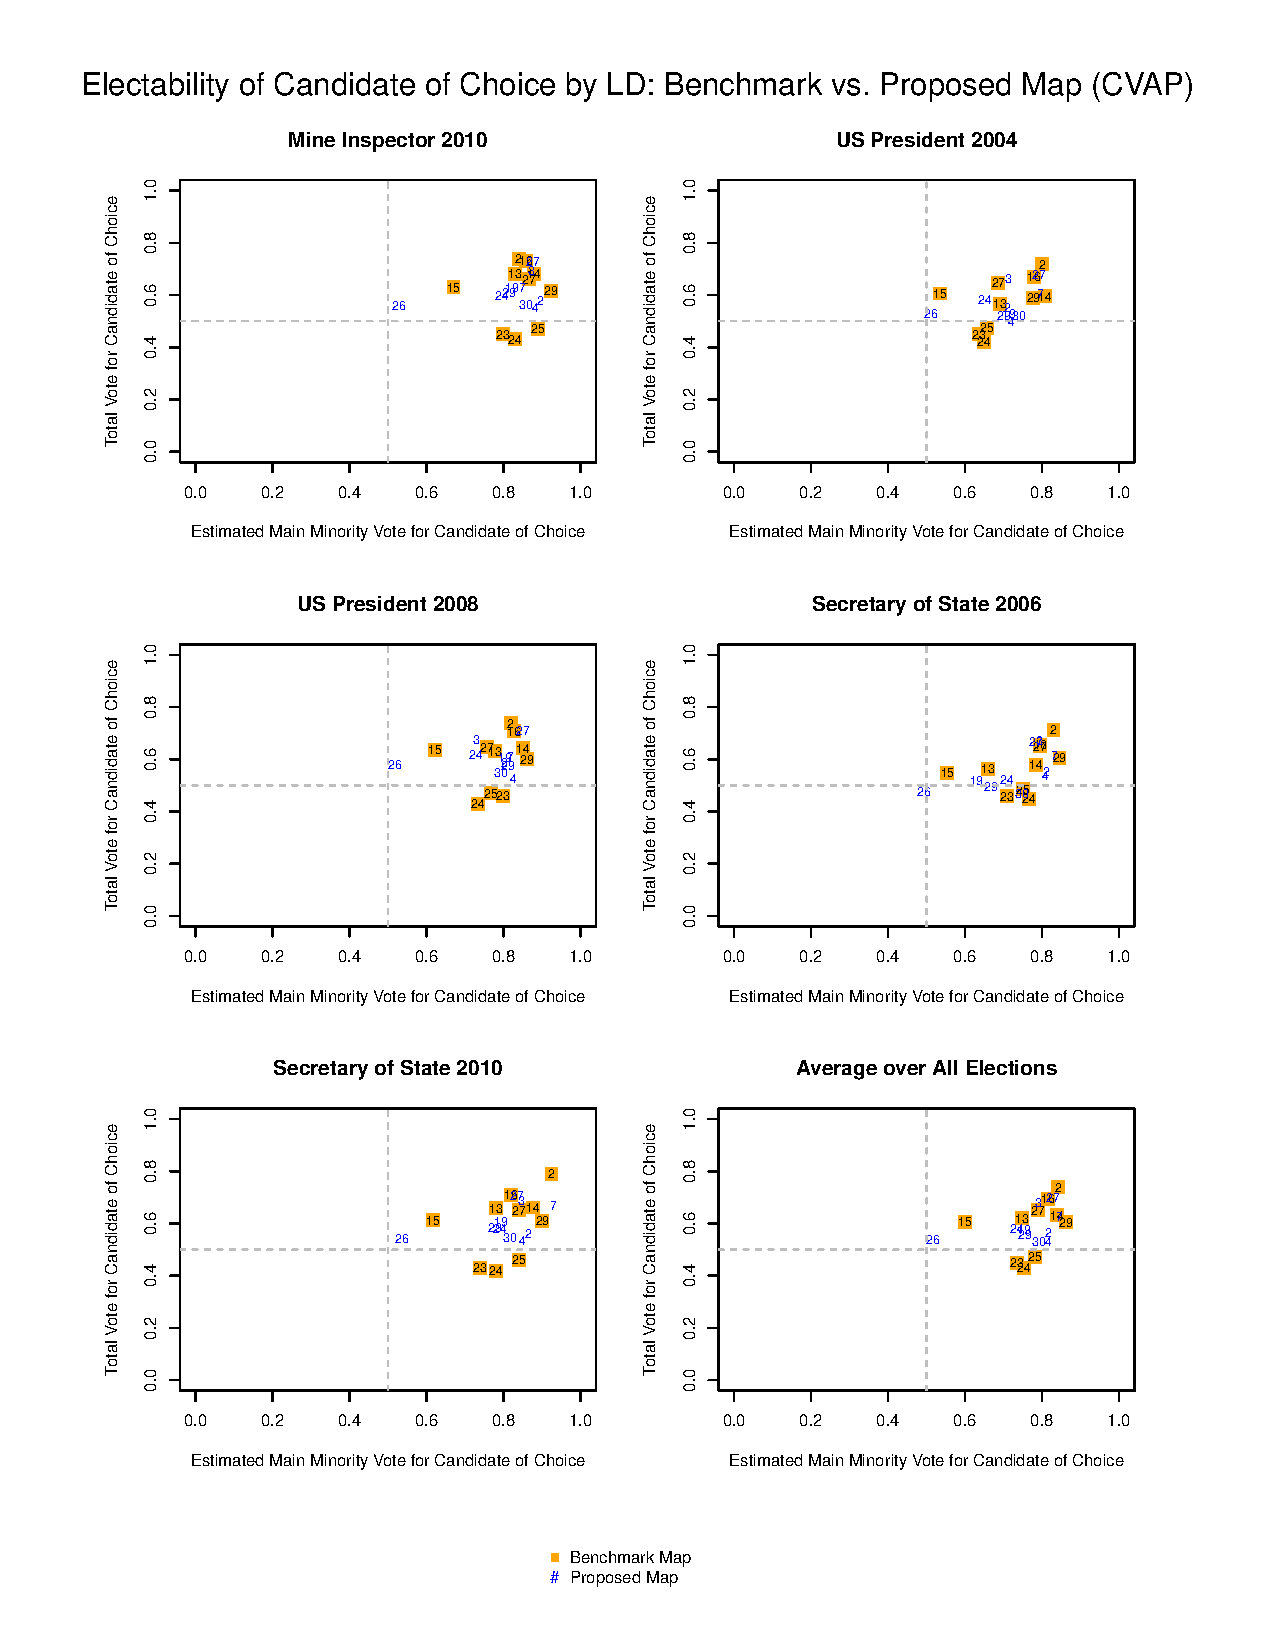
\includegraphics[scale=.8]{cvap_ld.pdf}
\caption{CVAP Legislative Districts}
\end{centering}
\end{figure}

\subsection{The Potential for Stronger Districts: A Counterfactual Analysis}

\begin{figure}[ht]
\begin{centering}
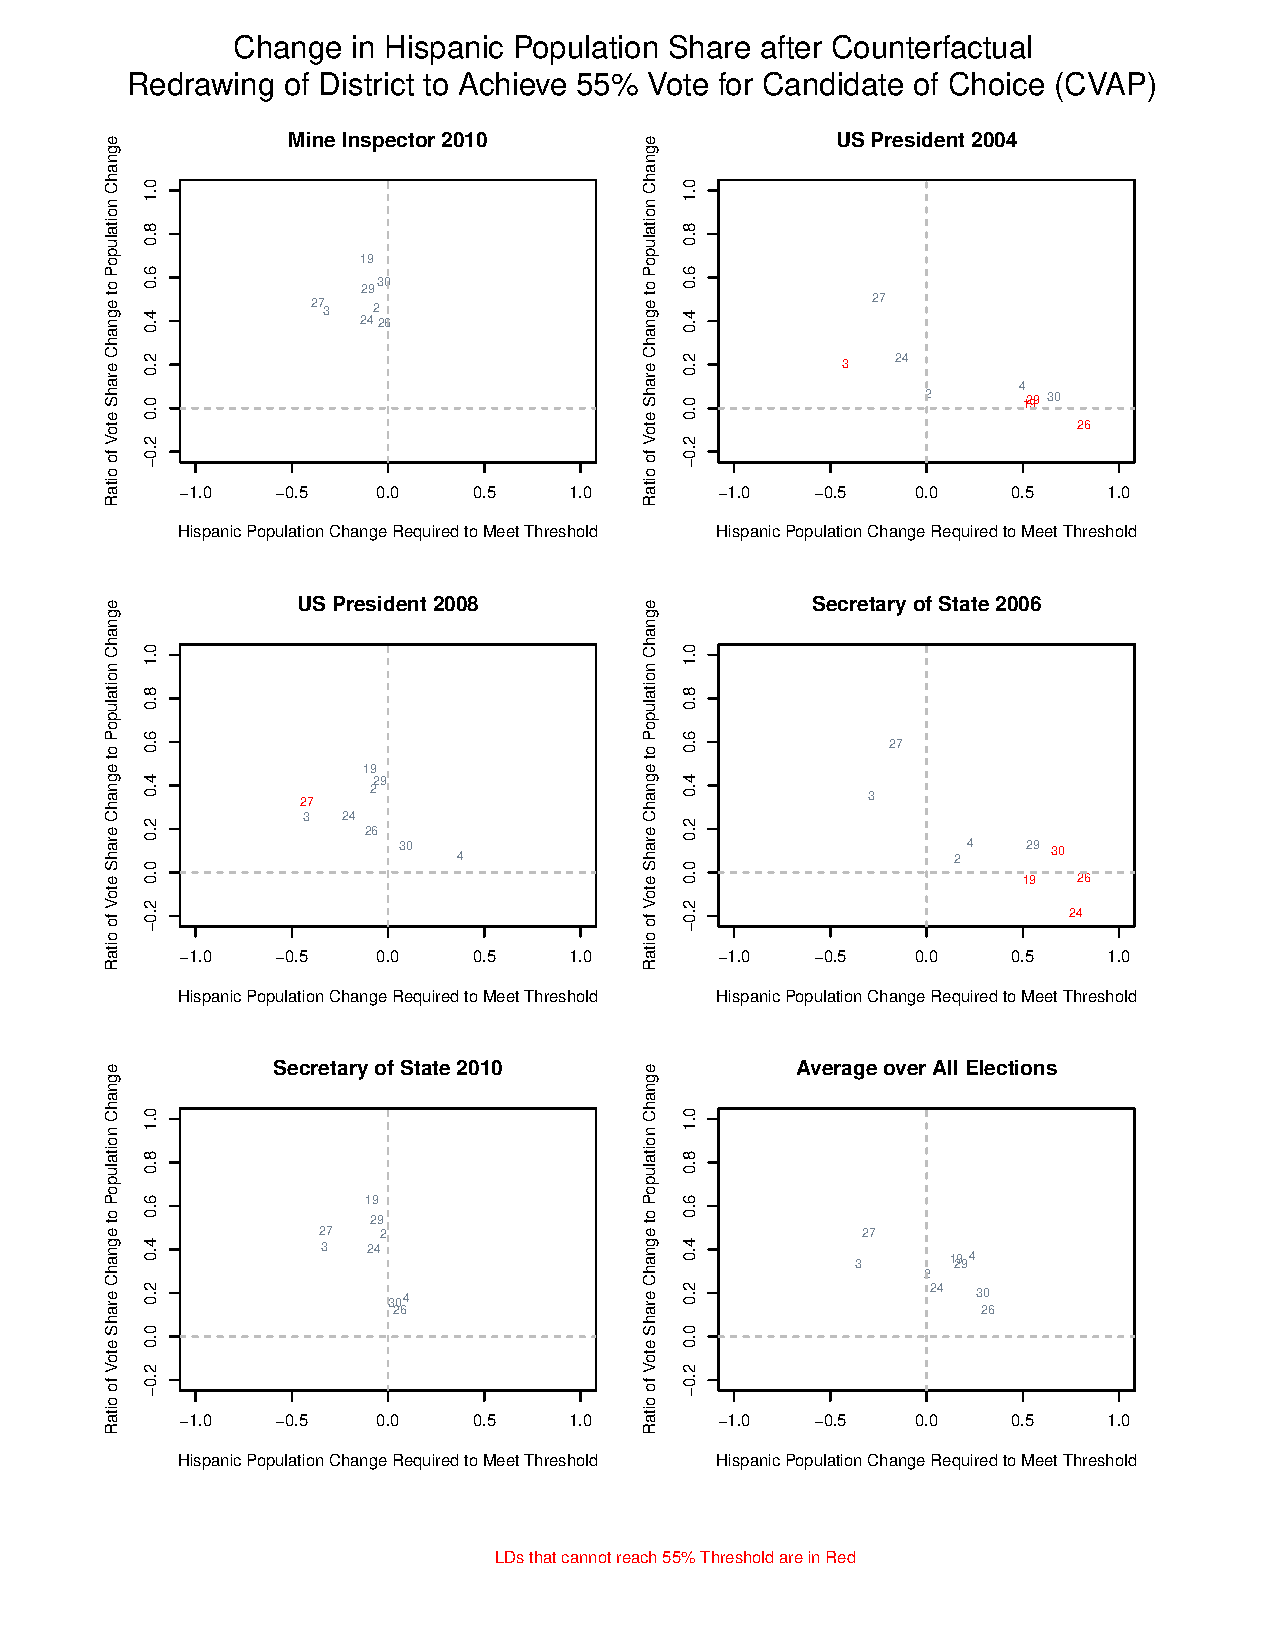
\includegraphics[scale=.8]{cvap_ld_performance_ratio.pdf}
\caption{CVAP Legislative Districts}
\end{centering}
\end{figure}

\section{Conclusion}

\singlespacing

\newpage
\bibliographystyle{apsr}

\bibliography{az_bib}

\appendix
\renewcommand*\appendixpagename{\section*{Appendix}}
\appendixpage

\section{Ecological Inference Estimates: CVAP CD}
\subsection{Proposed Map}

% latex table generated in R 2.13.1 by xtable 1.6-0 package
% Thu Jan 26 11:22:20 2012
\begin{table}[htb]
\begin{center}
\caption{Mine Inspector 2010 CD 3 (Proposed)}
\label{smine_cvap_cd_3}
\begin{tabular}{lccccc}
  \hline
Racial Group & Turnout & D Vote & R Vote & S Vote & Total CVAP \\ 
  \hline
White & 0.36 & 0.35 & 0.65 & 0.00 & 0.43 \\ 
  Hispanic & 0.30 & 0.90 & 0.10 & 0.00 & 0.44 \\ 
  Native American & 0.22 & 0.90 & 0.09 & 0.01 & 0.04 \\ 
  Black & 0.13 & 0.50 & 0.48 & 0.02 & 0.05 \\ 
  Other & 0.21 & 0.55 & 0.44 & 0.01 & 0.05 \\ 
  Total Pop & 0.31 & 0.61 & 0.39 & 0.00 &  \\ 
   \hline
\end{tabular}
\end{center}
\end{table}

% latex table generated in R 2.13.1 by xtable 1.6-0 package
% Thu Jan 26 11:22:20 2012
\begin{table}[htb]
\begin{center}
\caption{Mine Inspector 2010 CD 7 (Proposed)}
\label{smine_cvap_cd_7}
\begin{tabular}{lccccc}
  \hline
Racial Group & Turnout & D Vote & R Vote & S Vote & Total CVAP \\ 
  \hline
White & 0.33 & 0.50 & 0.50 & 0.00 & 0.39 \\ 
  Hispanic & 0.20 & 0.90 & 0.10 & 0.00 & 0.42 \\ 
  Native American & 0.13 & 0.67 & 0.30 & 0.03 & 0.03 \\ 
  Black & 0.24 & 0.80 & 0.20 & 0.01 & 0.10 \\ 
  Other & 0.26 & 0.72 & 0.26 & 0.01 & 0.06 \\ 
  Total Pop & 0.25 & 0.68 & 0.32 & 0.00 &  \\ 
   \hline
\end{tabular}
\end{center}
\end{table}


% latex table generated in R 2.13.1 by xtable 1.6-0 package
% Thu Jan 26 11:22:20 2012
\begin{table}[htb]
\begin{center}
\caption{US President 2004 CD 3 (Proposed)}
\label{pres04_cvap_cd_3}
\begin{tabular}{lccccc}
  \hline
Racial Group & Turnout & D Vote & R Vote & S Vote & Total CVAP \\ 
  \hline
White & 0.36 & 0.45 & 0.55 & 0.00 & 0.43 \\ 
  Hispanic & 0.41 & 0.69 & 0.30 & 0.00 & 0.44 \\ 
  Native American & 0.44 & 0.67 & 0.31 & 0.02 & 0.04 \\ 
  Black & 0.17 & 0.35 & 0.60 & 0.05 & 0.05 \\ 
  Other & 0.22 & 0.33 & 0.62 & 0.05 & 0.05 \\ 
  Total Pop & 0.37 & 0.57 & 0.42 & 0.01 &  \\ 
   \hline
\end{tabular}
\end{center}
\end{table}

% latex table generated in R 2.13.1 by xtable 1.6-0 package
% Thu Jan 26 11:22:20 2012
\begin{table}[htb]
\begin{center}
\caption{US President 2004 CD 7 (Proposed)}
\label{pres04_cvap_cd_7}
\begin{tabular}{lccccc}
  \hline
Racial Group & Turnout & D Vote & R Vote & S Vote & Total CVAP \\ 
  \hline
White & 0.44 & 0.49 & 0.50 & 0.00 & 0.39 \\ 
  Hispanic & 0.30 & 0.76 & 0.23 & 0.01 & 0.42 \\ 
  Native American & 0.21 & 0.48 & 0.46 & 0.06 & 0.03 \\ 
  Black & 0.22 & 0.61 & 0.36 & 0.03 & 0.10 \\ 
  Other & 0.12 & 0.40 & 0.52 & 0.08 & 0.06 \\ 
  Total Pop & 0.34 & 0.60 & 0.39 & 0.01 &  \\ 
   \hline
\end{tabular}
\end{center}
\end{table}


% latex table generated in R 2.13.1 by xtable 1.6-0 package
% Thu Jan 26 11:22:20 2012
\begin{table}[htb]
\begin{center}
\caption{US President 2008 CD 3 (Proposed)}
\label{pres08_cvap_cd_3}
\begin{tabular}{lccccc}
  \hline
Racial Group & Turnout & D Vote & R Vote & S Vote & Total CVAP \\ 
  \hline
White & 0.50 & 0.40 & 0.59 & 0.01 & 0.42 \\ 
  Hispanic & 0.42 & 0.79 & 0.20 & 0.01 & 0.44 \\ 
  Native American & 0.37 & 0.76 & 0.21 & 0.03 & 0.04 \\ 
  Black & 0.21 & 0.52 & 0.39 & 0.09 & 0.05 \\ 
  Other & 0.30 & 0.55 & 0.36 & 0.09 & 0.05 \\ 
  Total Pop & 0.43 & 0.59 & 0.40 & 0.01 &  \\ 
   \hline
\end{tabular}
\end{center}
\end{table}

% latex table generated in R 2.13.1 by xtable 1.6-0 package
% Thu Jan 26 11:22:20 2012
\begin{table}[htb]
\begin{center}
\caption{US President 2008 CD 7 (Proposed)}
\label{pres08_cvap_cd_7}
\begin{tabular}{lccccc}
  \hline
Racial Group & Turnout & D Vote & R Vote & S Vote & Total CVAP \\ 
  \hline
White & 0.50 & 0.51 & 0.48 & 0.01 & 0.39 \\ 
  Hispanic & 0.24 & 0.83 & 0.15 & 0.02 & 0.42 \\ 
  Native American & 0.24 & 0.53 & 0.39 & 0.08 & 0.03 \\ 
  Black & 0.48 & 0.83 & 0.15 & 0.03 & 0.10 \\ 
  Other & 0.49 & 0.61 & 0.34 & 0.05 & 0.06 \\ 
  Total Pop & 0.38 & 0.64 & 0.34 & 0.02 &  \\ 
   \hline
\end{tabular}
\end{center}
\end{table}


% latex table generated in R 2.13.1 by xtable 1.6-0 package
% Thu Jan 26 11:22:20 2012
\begin{table}[htb]
\begin{center}
\caption{Secretary of State 2006 CD 3 (Proposed)}
\label{sos06_cvap_cd_3}
\begin{tabular}{lccccc}
  \hline
Racial Group & Turnout & D Vote & R Vote & S Vote & Total CVAP \\ 
  \hline
White & 0.27 & 0.40 & 0.58 & 0.02 & 0.43 \\ 
  Hispanic & 0.26 & 0.77 & 0.21 & 0.02 & 0.44 \\ 
  Native American & 0.30 & 0.73 & 0.22 & 0.05 & 0.04 \\ 
  Black & 0.18 & 0.40 & 0.47 & 0.14 & 0.05 \\ 
  Other & 0.23 & 0.41 & 0.43 & 0.16 & 0.05 \\ 
  Total Pop & 0.26 & 0.58 & 0.39 & 0.03 &  \\ 
   \hline
\end{tabular}
\end{center}
\end{table}

% latex table generated in R 2.13.1 by xtable 1.6-0 package
% Thu Jan 26 11:22:20 2012
\begin{table}[htb]
\begin{center}
\caption{Secretary of State 2006 CD 7 (Proposed)}
\label{sos06_cvap_cd_7}
\begin{tabular}{lccccc}
  \hline
Racial Group & Turnout & D Vote & R Vote & S Vote & Total CVAP \\ 
  \hline
White & 0.32 & 0.46 & 0.52 & 0.02 & 0.39 \\ 
  Hispanic & 0.17 & 0.76 & 0.20 & 0.04 & 0.42 \\ 
  Native American & 0.16 & 0.46 & 0.37 & 0.17 & 0.03 \\ 
  Black & 0.18 & 0.52 & 0.38 & 0.10 & 0.10 \\ 
  Other & 0.14 & 0.46 & 0.35 & 0.20 & 0.06 \\ 
  Total Pop & 0.23 & 0.56 & 0.40 & 0.04 &  \\ 
   \hline
\end{tabular}
\end{center}
\end{table}


% latex table generated in R 2.13.1 by xtable 1.6-0 package
% Thu Jan 26 11:22:20 2012
\begin{table}[htb]
\begin{center}
\caption{Secretary of State 2010 CD 3 (Proposed)}
\label{sos10_cvap_cd_3}
\begin{tabular}{lccccc}
  \hline
Racial Group & Turnout & D Vote & R Vote & S Vote & Total CVAP \\ 
  \hline
White & 0.37 & 0.34 & 0.66 & 0.00 & 0.43 \\ 
  Hispanic & 0.31 & 0.87 & 0.13 & 0.00 & 0.44 \\ 
  Native American & 0.23 & 0.91 & 0.08 & 0.01 & 0.04 \\ 
  Black & 0.14 & 0.48 & 0.50 & 0.02 & 0.05 \\ 
  Other & 0.23 & 0.65 & 0.34 & 0.01 & 0.05 \\ 
  Total Pop & 0.32 & 0.60 & 0.40 & 0.00 &  \\ 
   \hline
\end{tabular}
\end{center}
\end{table}

% latex table generated in R 2.13.1 by xtable 1.6-0 package
% Thu Jan 26 11:22:20 2012
\begin{table}[htb]
\begin{center}
\caption{Secretary of State 2010 CD 7 (Proposed)}
\label{sos10_cvap_cd_7}
\begin{tabular}{lccccc}
  \hline
Racial Group & Turnout & D Vote & R Vote & S Vote & Total CVAP \\ 
  \hline
White & 0.34 & 0.49 & 0.51 & 0.00 & 0.39 \\ 
  Hispanic & 0.19 & 0.88 & 0.12 & 0.00 & 0.42 \\ 
  Native American & 0.15 & 0.73 & 0.24 & 0.03 & 0.03 \\ 
  Black & 0.26 & 0.79 & 0.20 & 0.01 & 0.10 \\ 
  Other & 0.26 & 0.68 & 0.30 & 0.01 & 0.06 \\ 
  Total Pop & 0.26 & 0.66 & 0.34 & 0.00 &  \\ 
   \hline
\end{tabular}
\end{center}
\end{table}


\subsection{Benchmark Map}
\clearpage

% latex table generated in R 2.13.1 by xtable 1.6-0 package
% Thu Jan 26 11:22:20 2012
\begin{table}[htb]
\begin{center}
\caption{Mine Inspector 2010 CD 4 (Benchmark)}
\label{smine_cvap_cd_4_benchmark}
\begin{tabular}{lccccc}
  \hline
Racial Group & Turnout & D Vote & R Vote & S Vote & Total CVAP \\ 
  \hline
White & 0.34 & 0.56 & 0.44 & 0.00 & 0.40 \\ 
  Hispanic & 0.19 & 0.89 & 0.11 & 0.00 & 0.41 \\ 
  Native American & 0.13 & 0.65 & 0.32 & 0.03 & 0.03 \\ 
  Black & 0.23 & 0.82 & 0.17 & 0.01 & 0.10 \\ 
  Other & 0.30 & 0.58 & 0.41 & 0.01 & 0.06 \\ 
  Total Votes & 0.26 & 0.68 & 0.31 & 0.00 &  \\ 
   \hline
\end{tabular}
\end{center}
\end{table}

% latex table generated in R 2.13.1 by xtable 1.6-0 package
% Thu Jan 26 11:22:20 2012
\begin{table}[htb]
\begin{center}
\caption{Mine Inspector 2010 CD 7 (Benchmark)}
\label{smine_cvap_cd_7_benchmark}
\begin{tabular}{lccccc}
  \hline
Racial Group & Turnout & D Vote & R Vote & S Vote & Total CVAP \\ 
  \hline
White & 0.32 & 0.33 & 0.67 & 0.00 & 0.47 \\ 
  Hispanic & 0.31 & 0.89 & 0.11 & 0.00 & 0.39 \\ 
  Native American & 0.16 & 0.89 & 0.10 & 0.01 & 0.05 \\ 
  Black & 0.16 & 0.54 & 0.44 & 0.01 & 0.04 \\ 
  Other & 0.37 & 0.67 & 0.32 & 0.01 & 0.05 \\ 
  Total Votes & 0.30 & 0.59 & 0.41 & 0.00 &  \\ 
   \hline
\end{tabular}
\end{center}
\end{table}


% latex table generated in R 2.13.1 by xtable 1.6-0 package
% Thu Jan 26 11:22:20 2012
\begin{table}[htb]
\begin{center}
\caption{US President 2004 CD 4 (Benchmark)}
\label{pres04_cvap_cd_4_benchmark}
\begin{tabular}{lccccc}
  \hline
Racial Group & Turnout & D Vote & R Vote & S Vote & Total CVAP \\ 
  \hline
White & 0.43 & 0.55 & 0.45 & 0.00 & 0.40 \\ 
  Hispanic & 0.31 & 0.73 & 0.26 & 0.01 & 0.41 \\ 
  Native American & 0.24 & 0.48 & 0.47 & 0.05 & 0.03 \\ 
  Black & 0.21 & 0.59 & 0.38 & 0.02 & 0.10 \\ 
  Other & 0.15 & 0.42 & 0.51 & 0.07 & 0.06 \\ 
  Total Votes & 0.34 & 0.61 & 0.38 & 0.01 &  \\ 
   \hline
\end{tabular}
\end{center}
\end{table}

% latex table generated in R 2.13.1 by xtable 1.6-0 package
% Thu Jan 26 11:22:21 2012
\begin{table}[htb]
\begin{center}
\caption{US President 2004 CD 7 (Benchmark)}
\label{pres04_cvap_cd_7_benchmark}
\begin{tabular}{lccccc}
  \hline
Racial Group & Turnout & D Vote & R Vote & S Vote & Total CVAP \\ 
  \hline
White & 0.37 & 0.45 & 0.54 & 0.00 & 0.47 \\ 
  Hispanic & 0.41 & 0.70 & 0.30 & 0.00 & 0.39 \\ 
  Native American & 0.26 & 0.62 & 0.35 & 0.03 & 0.05 \\ 
  Black & 0.18 & 0.56 & 0.39 & 0.05 & 0.04 \\ 
  Other & 0.35 & 0.44 & 0.53 & 0.03 & 0.05 \\ 
  Total Votes & 0.37 & 0.57 & 0.43 & 0.01 &  \\ 
   \hline
\end{tabular}
\end{center}
\end{table}


% latex table generated in R 2.13.1 by xtable 1.6-0 package
% Thu Jan 26 11:22:21 2012
\begin{table}[htb]
\begin{center}
\caption{US President 2008 CD 4 (Benchmark)}
\label{pres08_cvap_cd_4_benchmark}
\begin{tabular}{lccccc}
  \hline
Racial Group & Turnout & D Vote & R Vote & S Vote & Total CVAP \\ 
  \hline
White & 0.51 & 0.57 & 0.42 & 0.01 & 0.40 \\ 
  Hispanic & 0.23 & 0.82 & 0.17 & 0.02 & 0.41 \\ 
  Native American & 0.28 & 0.57 & 0.35 & 0.09 & 0.03 \\ 
  Black & 0.48 & 0.82 & 0.15 & 0.03 & 0.10 \\ 
  Other & 0.43 & 0.43 & 0.51 & 0.06 & 0.06 \\ 
  Total Votes & 0.38 & 0.65 & 0.33 & 0.02 &  \\ 
   \hline
\end{tabular}
\end{center}
\end{table}

% latex table generated in R 2.13.1 by xtable 1.6-0 package
% Thu Jan 26 11:22:21 2012
\begin{table}[htb]
\begin{center}
\caption{US President 2008 CD 7 (Benchmark)}
\label{pres08_cvap_cd_7_benchmark}
\begin{tabular}{lccccc}
  \hline
Racial Group & Turnout & D Vote & R Vote & S Vote & Total CVAP \\ 
  \hline
White & 0.43 & 0.39 & 0.61 & 0.01 & 0.47 \\ 
  Hispanic & 0.43 & 0.78 & 0.21 & 0.01 & 0.39 \\ 
  Native American & 0.28 & 0.71 & 0.26 & 0.03 & 0.05 \\ 
  Black & 0.32 & 0.57 & 0.36 & 0.07 & 0.04 \\ 
  Other & 0.49 & 0.61 & 0.34 & 0.05 & 0.05 \\ 
  Total Votes & 0.42 & 0.57 & 0.41 & 0.01 &  \\ 
   \hline
\end{tabular}
\end{center}
\end{table}


% latex table generated in R 2.13.1 by xtable 1.6-0 package
% Thu Jan 26 11:22:21 2012
\begin{table}[htb]
\begin{center}
\caption{Secretary of State 2006 CD 4 (Benchmark)}
\label{sos06_cvap_cd_4_benchmark}
\begin{tabular}{lccccc}
  \hline
Racial Group & Turnout & D Vote & R Vote & S Vote & Total CVAP \\ 
  \hline
White & 0.30 & 0.49 & 0.48 & 0.02 & 0.40 \\ 
  Hispanic & 0.17 & 0.72 & 0.25 & 0.03 & 0.41 \\ 
  Native American & 0.15 & 0.47 & 0.37 & 0.17 & 0.03 \\ 
  Black & 0.17 & 0.60 & 0.30 & 0.10 & 0.10 \\ 
  Other & 0.17 & 0.40 & 0.44 & 0.16 & 0.06 \\ 
  Total Votes & 0.22 & 0.57 & 0.39 & 0.04 &  \\ 
   \hline
\end{tabular}
\end{center}
\end{table}

% latex table generated in R 2.13.1 by xtable 1.6-0 package
% Thu Jan 26 11:22:21 2012
\begin{table}[htb]
\begin{center}
\caption{Secretary of State 2006 CD 7 (Benchmark)}
\label{sos06_cvap_cd_7_benchmark}
\begin{tabular}{lccccc}
  \hline
Racial Group & Turnout & D Vote & R Vote & S Vote & Total CVAP \\ 
  \hline
White & 0.27 & 0.41 & 0.56 & 0.02 & 0.47 \\ 
  Hispanic & 0.26 & 0.77 & 0.21 & 0.03 & 0.39 \\ 
  Native American & 0.20 & 0.66 & 0.27 & 0.07 & 0.05 \\ 
  Black & 0.18 & 0.51 & 0.34 & 0.15 & 0.04 \\ 
  Other & 0.22 & 0.33 & 0.49 & 0.17 & 0.05 \\ 
  Total Votes & 0.26 & 0.56 & 0.40 & 0.04 &  \\ 
   \hline
\end{tabular}
\end{center}
\end{table}


% latex table generated in R 2.13.1 by xtable 1.6-0 package
% Thu Jan 26 11:22:21 2012
\begin{table}[htb]
\begin{center}
\caption{Secretary of State 2010 CD 4 (Benchmark)}
\label{sos10_cvap_cd_4_benchmark}
\begin{tabular}{lccccc}
  \hline
Racial Group & Turnout & D Vote & R Vote & S Vote & Total CVAP \\ 
  \hline
White & 0.35 & 0.54 & 0.46 & 0.00 & 0.40 \\ 
  Hispanic & 0.19 & 0.88 & 0.12 & 0.00 & 0.41 \\ 
  Native American & 0.15 & 0.69 & 0.29 & 0.02 & 0.03 \\ 
  Black & 0.23 & 0.81 & 0.18 & 0.01 & 0.10 \\ 
  Other & 0.33 & 0.54 & 0.45 & 0.01 & 0.06 \\ 
  Total Votes & 0.26 & 0.67 & 0.33 & 0.00 &  \\ 
   \hline
\end{tabular}
\end{center}
\end{table}

% latex table generated in R 2.13.1 by xtable 1.6-0 package
% Thu Jan 26 11:22:21 2012
\begin{table}[htb]
\begin{center}
\caption{Secretary of State 2010 CD 7 (Benchmark)}
\label{sos10_cvap_cd_7_benchmark}
\begin{tabular}{lccccc}
  \hline
Racial Group & Turnout & D Vote & R Vote & S Vote & Total CVAP \\ 
  \hline
White & 0.33 & 0.34 & 0.66 & 0.00 & 0.47 \\ 
  Hispanic & 0.30 & 0.85 & 0.15 & 0.00 & 0.39 \\ 
  Native American & 0.17 & 0.89 & 0.11 & 0.01 & 0.05 \\ 
  Black & 0.18 & 0.48 & 0.51 & 0.01 & 0.04 \\ 
  Other & 0.36 & 0.76 & 0.23 & 0.01 & 0.05 \\ 
  Total Votes & 0.31 & 0.58 & 0.42 & 0.00 &  \\ 
   \hline
\end{tabular}
\end{center}
\end{table}



%\section{Ecological Inference Estimates: VAP CD}
%\subsection{Proposed Map}
%\clearpage

%% latex table generated in R 2.13.1 by xtable 1.6-0 package
% Thu Jan 26 11:22:21 2012
\begin{table}[htb]
\begin{center}
\caption{Mine Inspector 2010 CD 3 (Proposed)}
\label{smine_vap_cd_3}
\begin{tabular}{lccccc}
  \hline
Racial Group & Turnout & D Vote & R Vote & S Vote & Total VAP \\ 
  \hline
White & 0.40 & 0.38 & 0.62 & 0.00 & 0.35 \\ 
  Hispanic & 0.18 & 0.90 & 0.10 & 0.00 & 0.55 \\ 
  Native American & 0.23 & 0.90 & 0.09 & 0.01 & 0.03 \\ 
  Black & 0.10 & 0.60 & 0.37 & 0.03 & 0.04 \\ 
  Other & 0.16 & 0.66 & 0.32 & 0.02 & 0.03 \\ 
  Total Pop & 0.25 & 0.61 & 0.39 & 0.00 &  \\ 
   \hline
\end{tabular}
\end{center}
\end{table}

%% latex table generated in R 2.13.1 by xtable 1.6-0 package
% Thu Jan 26 11:22:21 2012
\begin{table}[htb]
\begin{center}
\caption{Mine Inspector 2010 CD 7 (Proposed)}
\label{smine_vap_cd_7}
\begin{tabular}{lccccc}
  \hline
Racial Group & Turnout & D Vote & R Vote & S Vote & Total VAP \\ 
  \hline
White & 0.38 & 0.55 & 0.45 & 0.00 & 0.27 \\ 
  Hispanic & 0.10 & 0.89 & 0.11 & 0.00 & 0.58 \\ 
  Native American & 0.28 & 0.86 & 0.12 & 0.02 & 0.02 \\ 
  Black & 0.17 & 0.81 & 0.18 & 0.01 & 0.09 \\ 
  Other & 0.24 & 0.49 & 0.50 & 0.01 & 0.04 \\ 
  Total Pop & 0.19 & 0.68 & 0.32 & 0.00 &  \\ 
   \hline
\end{tabular}
\end{center}
\end{table}


%% latex table generated in R 2.13.1 by xtable 1.6-0 package
% Thu Jan 26 11:22:21 2012
\begin{table}[htb]
\begin{center}
\caption{US President 2004 CD 3 (Proposed)}
\label{pres04_vap_cd_3}
\begin{tabular}{lccccc}
  \hline
Racial Group & Turnout & D Vote & R Vote & S Vote & Total VAP \\ 
  \hline
White & 0.35 & 0.47 & 0.52 & 0.00 & 0.34 \\ 
  Hispanic & 0.27 & 0.67 & 0.33 & 0.00 & 0.55 \\ 
  Native American & 0.44 & 0.63 & 0.35 & 0.02 & 0.03 \\ 
  Black & 0.19 & 0.41 & 0.55 & 0.04 & 0.04 \\ 
  Other & 0.22 & 0.38 & 0.57 & 0.05 & 0.03 \\ 
  Total Pop & 0.30 & 0.57 & 0.42 & 0.01 &  \\ 
   \hline
\end{tabular}
\end{center}
\end{table}

%% latex table generated in R 2.13.1 by xtable 1.6-0 package
% Thu Jan 26 11:22:21 2012
\begin{table}[htb]
\begin{center}
\caption{US President 2004 CD 7 (Proposed)}
\label{pres04_vap_cd_7}
\begin{tabular}{lccccc}
  \hline
Racial Group & Turnout & D Vote & R Vote & S Vote & Total VAP \\ 
  \hline
White & 0.48 & 0.51 & 0.49 & 0.00 & 0.27 \\ 
  Hispanic & 0.17 & 0.73 & 0.26 & 0.01 & 0.58 \\ 
  Native American & 0.25 & 0.47 & 0.47 & 0.06 & 0.02 \\ 
  Black & 0.13 & 0.59 & 0.37 & 0.04 & 0.09 \\ 
  Other & 0.12 & 0.40 & 0.52 & 0.08 & 0.04 \\ 
  Total Pop & 0.25 & 0.60 & 0.39 & 0.01 &  \\ 
   \hline
\end{tabular}
\end{center}
\end{table}


%% latex table generated in R 2.13.1 by xtable 1.6-0 package
% Thu Jan 26 11:22:21 2012
\begin{table}[htb]
\begin{center}
\caption{US President 2008 CD 3 (Proposed)}
\label{pres08_vap_cd_3}
\begin{tabular}{lccccc}
  \hline
Racial Group & Turnout & D Vote & R Vote & S Vote & Total VAP \\ 
  \hline
White & 0.54 & 0.41 & 0.58 & 0.01 & 0.35 \\ 
  Hispanic & 0.25 & 0.78 & 0.21 & 0.01 & 0.55 \\ 
  Native American & 0.37 & 0.75 & 0.22 & 0.03 & 0.03 \\ 
  Black & 0.22 & 0.59 & 0.34 & 0.07 & 0.04 \\ 
  Other & 0.43 & 0.74 & 0.19 & 0.07 & 0.03 \\ 
  Total Pop & 0.36 & 0.58 & 0.41 & 0.01 &  \\ 
   \hline
\end{tabular}
\end{center}
\end{table}

%% latex table generated in R 2.13.1 by xtable 1.6-0 package
% Thu Jan 26 11:22:21 2012
\begin{table}[htb]
\begin{center}
\caption{US President 2008 CD 7 (Proposed)}
\label{pres08_vap_cd_7}
\begin{tabular}{lccccc}
  \hline
Racial Group & Turnout & D Vote & R Vote & S Vote & Total VAP \\ 
  \hline
White & 0.58 & 0.55 & 0.45 & 0.01 & 0.27 \\ 
  Hispanic & 0.12 & 0.80 & 0.18 & 0.02 & 0.58 \\ 
  Native American & 0.41 & 0.64 & 0.28 & 0.08 & 0.02 \\ 
  Black & 0.40 & 0.84 & 0.13 & 0.03 & 0.09 \\ 
  Other & 0.35 & 0.47 & 0.47 & 0.07 & 0.04 \\ 
  Total Pop & 0.28 & 0.64 & 0.34 & 0.02 &  \\ 
   \hline
\end{tabular}
\end{center}
\end{table}


%% latex table generated in R 2.13.1 by xtable 1.6-0 package
% Thu Jan 26 11:22:21 2012
\begin{table}[htb]
\begin{center}
\caption{Secretary of State 2006 CD 3 (Proposed)}
\label{sos06_vap_cd_3}
\begin{tabular}{lccccc}
  \hline
Racial Group & Turnout & D Vote & R Vote & S Vote & Total VAP \\ 
  \hline
White & 0.28 & 0.39 & 0.58 & 0.03 & 0.34 \\ 
  Hispanic & 0.16 & 0.78 & 0.20 & 0.02 & 0.55 \\ 
  Native American & 0.32 & 0.69 & 0.25 & 0.06 & 0.03 \\ 
  Black & 0.15 & 0.38 & 0.46 & 0.16 & 0.04 \\ 
  Other & 0.21 & 0.43 & 0.40 & 0.17 & 0.03 \\ 
  Total Pop & 0.21 & 0.57 & 0.39 & 0.03 &  \\ 
   \hline
\end{tabular}
\end{center}
\end{table}

%% latex table generated in R 2.13.1 by xtable 1.6-0 package
% Thu Jan 26 11:22:21 2012
\begin{table}[htb]
\begin{center}
\caption{Secretary of State 2006 CD 7 (Proposed)}
\label{sos06_vap_cd_7}
\begin{tabular}{lccccc}
  \hline
Racial Group & Turnout & D Vote & R Vote & S Vote & Total VAP \\ 
  \hline
White & 0.35 & 0.46 & 0.52 & 0.02 & 0.27 \\ 
  Hispanic & 0.09 & 0.75 & 0.21 & 0.04 & 0.58 \\ 
  Native American & 0.22 & 0.49 & 0.34 & 0.18 & 0.02 \\ 
  Black & 0.13 & 0.50 & 0.39 & 0.11 & 0.09 \\ 
  Other & 0.14 & 0.43 & 0.38 & 0.19 & 0.04 \\ 
  Total Pop & 0.17 & 0.56 & 0.40 & 0.04 &  \\ 
   \hline
\end{tabular}
\end{center}
\end{table}


%% latex table generated in R 2.13.1 by xtable 1.6-0 package
% Thu Jan 26 11:22:21 2012
\begin{table}[htb]
\begin{center}
\caption{Secretary of State 2010 CD 3 (Proposed)}
\label{sos10_vap_cd_3}
\begin{tabular}{lccccc}
  \hline
Racial Group & Turnout & D Vote & R Vote & S Vote & Total VAP \\ 
  \hline
White & 0.41 & 0.38 & 0.62 & 0.00 & 0.35 \\ 
  Hispanic & 0.18 & 0.87 & 0.13 & 0.00 & 0.55 \\ 
  Native American & 0.23 & 0.91 & 0.08 & 0.01 & 0.03 \\ 
  Black & 0.11 & 0.59 & 0.38 & 0.02 & 0.04 \\ 
  Other & 0.18 & 0.71 & 0.28 & 0.02 & 0.03 \\ 
  Total Pop & 0.25 & 0.59 & 0.41 & 0.00 &  \\ 
   \hline
\end{tabular}
\end{center}
\end{table}

%% latex table generated in R 2.13.1 by xtable 1.6-0 package
% Thu Jan 26 11:22:21 2012
\begin{table}[htb]
\begin{center}
\caption{Secretary of State 2010 CD 7 (Proposed)}
\label{sos10_vap_cd_7}
\begin{tabular}{lccccc}
  \hline
Racial Group & Turnout & D Vote & R Vote & S Vote & Total VAP \\ 
  \hline
White & 0.40 & 0.52 & 0.47 & 0.00 & 0.27 \\ 
  Hispanic & 0.09 & 0.88 & 0.12 & 0.00 & 0.58 \\ 
  Native American & 0.29 & 0.81 & 0.17 & 0.02 & 0.02 \\ 
  Black & 0.19 & 0.81 & 0.18 & 0.01 & 0.09 \\ 
  Other & 0.24 & 0.52 & 0.47 & 0.01 & 0.04 \\ 
  Total Pop & 0.19 & 0.66 & 0.34 & 0.00 &  \\ 
   \hline
\end{tabular}
\end{center}
\end{table}


%\subsection{Benchmark Map}
%\clearpage
%% latex table generated in R 2.13.1 by xtable 1.6-0 package
% Thu Jan 26 11:22:21 2012
\begin{table}[htb]
\begin{center}
\caption{Mine Inspector 2010 CD 4 (Benchmark)}
\label{smine_vap_cd_4_benchmark}
\begin{tabular}{lccccc}
  \hline
Racial Group & Turnout & D Vote & R Vote & S Vote & Total VAP \\ 
  \hline
White & 0.39 & 0.58 & 0.42 & 0.00 & 0.27 \\ 
  Hispanic & 0.09 & 0.89 & 0.11 & 0.00 & 0.58 \\ 
  Native American & 0.28 & 0.83 & 0.16 & 0.02 & 0.02 \\ 
  Black & 0.17 & 0.83 & 0.16 & 0.01 & 0.09 \\ 
  Other & 0.24 & 0.44 & 0.55 & 0.02 & 0.04 \\ 
  Total Votes & 0.19 & 0.69 & 0.31 & 0.00 &  \\ 
   \hline
\end{tabular}
\end{center}
\end{table}

%% latex table generated in R 2.13.1 by xtable 1.6-0 package
% Thu Jan 26 11:22:21 2012
\begin{table}[htb]
\begin{center}
\caption{Mine Inspector 2010 CD 7 (Benchmark)}
\label{smine_vap_cd_7_benchmark}
\begin{tabular}{lccccc}
  \hline
Racial Group & Turnout & D Vote & R Vote & S Vote & Total VAP \\ 
  \hline
White & 0.36 & 0.36 & 0.64 & 0.00 & 0.39 \\ 
  Hispanic & 0.19 & 0.90 & 0.10 & 0.00 & 0.50 \\ 
  Native American & 0.17 & 0.87 & 0.12 & 0.01 & 0.04 \\ 
  Black & 0.14 & 0.52 & 0.47 & 0.01 & 0.04 \\ 
  Other & 0.18 & 0.67 & 0.32 & 0.01 & 0.03 \\ 
  Total Votes & 0.25 & 0.59 & 0.41 & 0.00 &  \\ 
   \hline
\end{tabular}
\end{center}
\end{table}


%% latex table generated in R 2.13.1 by xtable 1.6-0 package
% Thu Jan 26 11:22:21 2012
\begin{table}[htb]
\begin{center}
\caption{US President 2004 CD 4 (Benchmark)}
\label{pres04_vap_cd_4_benchmark}
\begin{tabular}{lccccc}
  \hline
Racial Group & Turnout & D Vote & R Vote & S Vote & Total VAP \\ 
  \hline
White & 0.47 & 0.54 & 0.46 & 0.00 & 0.27 \\ 
  Hispanic & 0.17 & 0.75 & 0.25 & 0.01 & 0.57 \\ 
  Native American & 0.27 & 0.46 & 0.48 & 0.06 & 0.02 \\ 
  Black & 0.15 & 0.55 & 0.42 & 0.03 & 0.09 \\ 
  Other & 0.13 & 0.49 & 0.45 & 0.07 & 0.04 \\ 
  Total Votes & 0.25 & 0.62 & 0.38 & 0.01 &  \\ 
   \hline
\end{tabular}
\end{center}
\end{table}

%% latex table generated in R 2.13.1 by xtable 1.6-0 package
% Thu Jan 26 11:22:21 2012
\begin{table}[htb]
\begin{center}
\caption{US President 2004 CD 7 (Benchmark)}
\label{pres04_vap_cd_7_benchmark}
\begin{tabular}{lccccc}
  \hline
Racial Group & Turnout & D Vote & R Vote & S Vote & Total VAP \\ 
  \hline
White & 0.38 & 0.48 & 0.51 & 0.00 & 0.39 \\ 
  Hispanic & 0.27 & 0.67 & 0.33 & 0.00 & 0.50 \\ 
  Native American & 0.26 & 0.61 & 0.36 & 0.03 & 0.04 \\ 
  Black & 0.16 & 0.45 & 0.50 & 0.05 & 0.04 \\ 
  Other & 0.24 & 0.46 & 0.50 & 0.04 & 0.03 \\ 
  Total Votes & 0.31 & 0.57 & 0.43 & 0.01 &  \\ 
   \hline
\end{tabular}
\end{center}
\end{table}


%% latex table generated in R 2.13.1 by xtable 1.6-0 package
% Thu Jan 26 11:22:21 2012
\begin{table}[htb]
\begin{center}
\caption{US President 2008 CD 4 (Benchmark)}
\label{pres08_vap_cd_4_benchmark}
\begin{tabular}{lccccc}
  \hline
Racial Group & Turnout & D Vote & R Vote & S Vote & Total VAP \\ 
  \hline
White & 0.59 & 0.56 & 0.43 & 0.01 & 0.27 \\ 
  Hispanic & 0.11 & 0.83 & 0.15 & 0.02 & 0.58 \\ 
  Native American & 0.46 & 0.64 & 0.27 & 0.09 & 0.02 \\ 
  Black & 0.39 & 0.84 & 0.13 & 0.03 & 0.09 \\ 
  Other & 0.36 & 0.46 & 0.48 & 0.06 & 0.04 \\ 
  Total Votes & 0.28 & 0.65 & 0.33 & 0.02 &  \\ 
   \hline
\end{tabular}
\end{center}
\end{table}

%% latex table generated in R 2.13.1 by xtable 1.6-0 package
% Thu Jan 26 11:22:21 2012
\begin{table}[htb]
\begin{center}
\caption{US President 2008 CD 7 (Benchmark)}
\label{pres08_vap_cd_7_benchmark}
\begin{tabular}{lccccc}
  \hline
Racial Group & Turnout & D Vote & R Vote & S Vote & Total VAP \\ 
  \hline
White & 0.48 & 0.41 & 0.58 & 0.01 & 0.39 \\ 
  Hispanic & 0.26 & 0.77 & 0.22 & 0.01 & 0.50 \\ 
  Native American & 0.30 & 0.70 & 0.27 & 0.03 & 0.04 \\ 
  Black & 0.29 & 0.66 & 0.28 & 0.06 & 0.04 \\ 
  Other & 0.47 & 0.63 & 0.31 & 0.07 & 0.03 \\ 
  Total Votes & 0.35 & 0.57 & 0.42 & 0.01 &  \\ 
   \hline
\end{tabular}
\end{center}
\end{table}


%% latex table generated in R 2.13.1 by xtable 1.6-0 package
% Thu Jan 26 11:22:21 2012
\begin{table}[htb]
\begin{center}
\caption{Secretary of State 2006 CD 4 (Benchmark)}
\label{sos06_vap_cd_4_benchmark}
\begin{tabular}{lccccc}
  \hline
Racial Group & Turnout & D Vote & R Vote & S Vote & Total VAP \\ 
  \hline
White & 0.33 & 0.49 & 0.49 & 0.02 & 0.27 \\ 
  Hispanic & 0.09 & 0.75 & 0.22 & 0.03 & 0.57 \\ 
  Native American & 0.21 & 0.48 & 0.35 & 0.17 & 0.02 \\ 
  Black & 0.12 & 0.49 & 0.39 & 0.12 & 0.09 \\ 
  Other & 0.15 & 0.41 & 0.42 & 0.17 & 0.04 \\ 
  Total Votes & 0.16 & 0.57 & 0.39 & 0.04 &  \\ 
   \hline
\end{tabular}
\end{center}
\end{table}

%% latex table generated in R 2.13.1 by xtable 1.6-0 package
% Thu Jan 26 11:22:21 2012
\begin{table}[htb]
\begin{center}
\caption{Secretary of State 2006 CD 7 (Benchmark)}
\label{sos06_vap_cd_7_benchmark}
\begin{tabular}{lccccc}
  \hline
Racial Group & Turnout & D Vote & R Vote & S Vote & Total VAP \\ 
  \hline
White & 0.28 & 0.42 & 0.56 & 0.02 & 0.39 \\ 
  Hispanic & 0.16 & 0.76 & 0.21 & 0.03 & 0.50 \\ 
  Native American & 0.21 & 0.63 & 0.30 & 0.07 & 0.04 \\ 
  Black & 0.16 & 0.45 & 0.39 & 0.16 & 0.04 \\ 
  Other & 0.22 & 0.40 & 0.42 & 0.18 & 0.03 \\ 
  Total Votes & 0.21 & 0.56 & 0.40 & 0.04 &  \\ 
   \hline
\end{tabular}
\end{center}
\end{table}


%% latex table generated in R 2.13.1 by xtable 1.6-0 package
% Thu Jan 26 11:22:21 2012
\begin{table}[htb]
\begin{center}
\caption{Secretary of State 2010 CD 4 (Benchmark)}
\label{sos10_vap_cd_4_benchmark}
\begin{tabular}{lccccc}
  \hline
Racial Group & Turnout & D Vote & R Vote & S Vote & Total VAP \\ 
  \hline
White & 0.40 & 0.56 & 0.44 & 0.00 & 0.27 \\ 
  Hispanic & 0.09 & 0.88 & 0.11 & 0.00 & 0.58 \\ 
  Native American & 0.28 & 0.78 & 0.20 & 0.02 & 0.02 \\ 
  Black & 0.19 & 0.81 & 0.18 & 0.01 & 0.09 \\ 
  Other & 0.26 & 0.46 & 0.53 & 0.01 & 0.04 \\ 
  Total Votes & 0.19 & 0.67 & 0.33 & 0.00 &  \\ 
   \hline
\end{tabular}
\end{center}
\end{table}

%% latex table generated in R 2.13.1 by xtable 1.6-0 package
% Thu Jan 26 11:22:21 2012
\begin{table}[htb]
\begin{center}
\caption{Secretary of State 2010 CD 7 (Benchmark)}
\label{sos10_vap_cd_7_benchmark}
\begin{tabular}{lccccc}
  \hline
Racial Group & Turnout & D Vote & R Vote & S Vote & Total VAP \\ 
  \hline
White & 0.37 & 0.37 & 0.63 & 0.00 & 0.39 \\ 
  Hispanic & 0.19 & 0.85 & 0.15 & 0.00 & 0.50 \\ 
  Native American & 0.17 & 0.90 & 0.09 & 0.01 & 0.04 \\ 
  Black & 0.15 & 0.63 & 0.36 & 0.01 & 0.04 \\ 
  Other & 0.17 & 0.67 & 0.32 & 0.01 & 0.03 \\ 
  Total Votes & 0.25 & 0.58 & 0.42 & 0.00 &  \\ 
   \hline
\end{tabular}
\end{center}
\end{table}


\section{CVAP LD}
\subsection{Proposed Map}
\clearpage

% latex table generated in R 2.13.1 by xtable 1.6-0 package
% Thu Jan 26 11:22:22 2012
\begin{table}[htb]
\begin{center}
\caption{Mine Inspector 2010 LD 2 (Proposed)}
\label{smine_cvap_ld_2}
\begin{tabular}{lccccc}
  \hline
Racial Group & Turnout & D Vote & R Vote & S Vote & Total CVAP \\ 
  \hline
White & 0.51 & 0.43 & 0.57 & 0.00 & 0.49 \\ 
  Hispanic & 0.28 & 0.89 & 0.10 & 0.00 & 0.41 \\ 
  Native American & 0.35 & 0.76 & 0.23 & 0.01 & 0.02 \\ 
  Black & 0.18 & 0.52 & 0.47 & 0.01 & 0.04 \\ 
  Other & 0.24 & 0.56 & 0.43 & 0.01 & 0.04 \\ 
  Total Pop & 0.39 & 0.58 & 0.42 & 0.00 &  \\ 
   \hline
\end{tabular}
\end{center}
\end{table}

% latex table generated in R 2.13.1 by xtable 1.6-0 package
% Thu Jan 26 11:22:22 2012
\begin{table}[htb]
\begin{center}
\caption{Mine Inspector 2010 LD 3 (Proposed)}
\label{smine_cvap_ld_3}
\begin{tabular}{lccccc}
  \hline
Racial Group & Turnout & D Vote & R Vote & S Vote & Total CVAP \\ 
  \hline
White & 0.33 & 0.53 & 0.47 & 0.00 & 0.45 \\ 
  Hispanic & 0.33 & 0.87 & 0.13 & 0.00 & 0.42 \\ 
  Native American & 0.21 & 0.74 & 0.25 & 0.01 & 0.04 \\ 
  Black & 0.30 & 0.64 & 0.35 & 0.01 & 0.03 \\ 
  Other & 0.45 & 0.65 & 0.34 & 0.00 & 0.05 \\ 
  Total Pop & 0.33 & 0.69 & 0.31 & 0.00 &  \\ 
   \hline
\end{tabular}
\end{center}
\end{table}

% latex table generated in R 2.13.1 by xtable 1.6-0 package
% Thu Jan 26 11:22:22 2012
\begin{table}[htb]
\begin{center}
\caption{Mine Inspector 2010 LD 4 (Proposed)}
\label{smine_cvap_ld_4}
\begin{tabular}{lccccc}
  \hline
Racial Group & Turnout & D Vote & R Vote & S Vote & Total CVAP \\ 
  \hline
White & 0.32 & 0.19 & 0.81 & 0.00 & 0.42 \\ 
  Hispanic & 0.28 & 0.88 & 0.12 & 0.00 & 0.42 \\ 
  Native American & 0.22 & 0.92 & 0.08 & 0.01 & 0.07 \\ 
  Black & 0.38 & 0.64 & 0.35 & 0.01 & 0.04 \\ 
  Other & 0.42 & 0.75 & 0.25 & 0.01 & 0.05 \\ 
  Total Pop & 0.30 & 0.55 & 0.45 & 0.00 &  \\ 
   \hline
\end{tabular}
\end{center}
\end{table}

% latex table generated in R 2.13.1 by xtable 1.6-0 package
% Thu Jan 26 11:22:22 2012
\begin{table}[htb]
\begin{center}
\caption{Mine Inspector 2010 LD 7 (Proposed)}
\label{smine_cvap_ld_7}
\begin{tabular}{lccccc}
  \hline
Racial Group & Turnout & D Vote & R Vote & S Vote & Total CVAP \\ 
  \hline
White & 0.44 & 0.23 & 0.77 & 0.00 & 0.28 \\ 
  Hispanic & 0.25 & 0.55 & 0.45 & 0.01 & 0.05 \\ 
  Native American & 0.34 & 0.85 & 0.15 & 0.00 & 0.63 \\ 
  Black & 0.41 & 0.56 & 0.42 & 0.02 & 0.01 \\ 
  Other & 0.28 & 0.80 & 0.19 & 0.01 & 0.04 \\ 
  Total Pop & 0.36 & 0.63 & 0.37 & 0.00 &  \\ 
   \hline
\end{tabular}
\end{center}
\end{table}

% latex table generated in R 2.13.1 by xtable 1.6-0 package
% Thu Jan 26 11:22:22 2012
\begin{table}[htb]
\begin{center}
\caption{Mine Inspector 2010 LD 8 (Proposed)}
\label{smine_cvap_ld_8}
\begin{tabular}{lccccc}
  \hline
Racial Group & Turnout & D Vote & R Vote & S Vote & Total CVAP \\ 
  \hline
White & 0.42 & 0.38 & 0.62 & 0.00 & 0.53 \\ 
  Hispanic & 0.18 & 0.83 & 0.17 & 0.00 & 0.30 \\ 
  Native American & 0.15 & 0.75 & 0.24 & 0.01 & 0.07 \\ 
  Black & 0.22 & 0.42 & 0.57 & 0.01 & 0.04 \\ 
  Other & 0.21 & 0.51 & 0.49 & 0.01 & 0.06 \\ 
  Total Pop & 0.31 & 0.48 & 0.52 & 0.00 &  \\ 
   \hline
\end{tabular}
\end{center}
\end{table}

% latex table generated in R 2.13.1 by xtable 1.6-0 package
% Thu Jan 26 11:22:22 2012
\begin{table}[htb]
\begin{center}
\caption{Mine Inspector 2010 LD 19 (Proposed)}
\label{smine_cvap_ld_19}
\begin{tabular}{lccccc}
  \hline
Racial Group & Turnout & D Vote & R Vote & S Vote & Total CVAP \\ 
  \hline
White & 0.22 & 0.38 & 0.62 & 0.00 & 0.38 \\ 
  Hispanic & 0.20 & 0.82 & 0.18 & 0.00 & 0.47 \\ 
  Native American & 0.20 & 0.47 & 0.50 & 0.04 & 0.02 \\ 
  Black & 0.45 & 0.66 & 0.33 & 0.00 & 0.09 \\ 
  Other & 0.48 & 0.67 & 0.33 & 0.01 & 0.05 \\ 
  Total Pop & 0.24 & 0.63 & 0.37 & 0.00 &  \\ 
   \hline
\end{tabular}
\end{center}
\end{table}

% latex table generated in R 2.13.1 by xtable 1.6-0 package
% Thu Jan 26 11:22:22 2012
\begin{table}[htb]
\begin{center}
\caption{Mine Inspector 2010 LD 24 (Proposed)}
\label{smine_cvap_ld_24}
\begin{tabular}{lccccc}
  \hline
Racial Group & Turnout & D Vote & R Vote & S Vote & Total CVAP \\ 
  \hline
White & 0.35 & 0.55 & 0.45 & 0.00 & 0.64 \\ 
  Hispanic & 0.14 & 0.79 & 0.20 & 0.01 & 0.22 \\ 
  Native American & 0.22 & 0.59 & 0.39 & 0.02 & 0.04 \\ 
  Black & 0.33 & 0.68 & 0.31 & 0.01 & 0.05 \\ 
  Other & 0.46 & 0.68 & 0.31 & 0.01 & 0.05 \\ 
  Total Pop & 0.30 & 0.60 & 0.40 & 0.00 &  \\ 
   \hline
\end{tabular}
\end{center}
\end{table}

% latex table generated in R 2.13.1 by xtable 1.6-0 package
% Thu Jan 26 11:22:22 2012
\begin{table}[htb]
\begin{center}
\caption{Mine Inspector 2010 LD 26 (Proposed)}
\label{smine_cvap_ld_26}
\begin{tabular}{lccccc}
  \hline
Racial Group & Turnout & D Vote & R Vote & S Vote & Total CVAP \\ 
  \hline
White & 0.27 & 0.55 & 0.45 & 0.00 & 0.65 \\ 
  Hispanic & 0.15 & 0.52 & 0.47 & 0.01 & 0.18 \\ 
  Native American & 0.31 & 0.65 & 0.34 & 0.01 & 0.06 \\ 
  Black & 0.29 & 0.59 & 0.40 & 0.01 & 0.05 \\ 
  Other & 0.29 & 0.58 & 0.40 & 0.01 & 0.06 \\ 
  Total Pop & 0.25 & 0.56 & 0.44 & 0.00 &  \\ 
   \hline
\end{tabular}
\end{center}
\end{table}

% latex table generated in R 2.13.1 by xtable 1.6-0 package
% Thu Jan 26 11:22:22 2012
\begin{table}[htb]
\begin{center}
\caption{Mine Inspector 2010 LD 27 (Proposed)}
\label{smine_cvap_ld_27}
\begin{tabular}{lccccc}
  \hline
Racial Group & Turnout & D Vote & R Vote & S Vote & Total CVAP \\ 
  \hline
White & 0.30 & 0.54 & 0.46 & 0.00 & 0.30 \\ 
  Hispanic & 0.21 & 0.87 & 0.12 & 0.00 & 0.42 \\ 
  Native American & 0.15 & 0.80 & 0.18 & 0.02 & 0.05 \\ 
  Black & 0.33 & 0.79 & 0.21 & 0.00 & 0.18 \\ 
  Other & 0.40 & 0.68 & 0.31 & 0.01 & 0.06 \\ 
  Total Pop & 0.26 & 0.73 & 0.27 & 0.00 &  \\ 
   \hline
\end{tabular}
\end{center}
\end{table}

% latex table generated in R 2.13.1 by xtable 1.6-0 package
% Thu Jan 26 11:22:22 2012
\begin{table}[htb]
\begin{center}
\caption{Mine Inspector 2010 LD 29 (Proposed)}
\label{smine_cvap_ld_29}
\begin{tabular}{lccccc}
  \hline
Racial Group & Turnout & D Vote & R Vote & S Vote & Total CVAP \\ 
  \hline
White & 0.26 & 0.42 & 0.58 & 0.00 & 0.41 \\ 
  Hispanic & 0.19 & 0.81 & 0.18 & 0.00 & 0.45 \\ 
  Native American & 0.60 & 0.55 & 0.43 & 0.02 & 0.01 \\ 
  Black & 0.42 & 0.65 & 0.34 & 0.01 & 0.08 \\ 
  Other & 0.44 & 0.65 & 0.34 & 0.01 & 0.05 \\ 
  Total Pop & 0.26 & 0.61 & 0.39 & 0.00 &  \\ 
   \hline
\end{tabular}
\end{center}
\end{table}

% latex table generated in R 2.13.1 by xtable 1.6-0 package
% Thu Jan 26 11:22:22 2012
\begin{table}[htb]
\begin{center}
\caption{Mine Inspector 2010 LD 30 (Proposed)}
\label{smine_cvap_ld_30}
\begin{tabular}{lccccc}
  \hline
Racial Group & Turnout & D Vote & R Vote & S Vote & Total CVAP \\ 
  \hline
White & 0.24 & 0.38 & 0.61 & 0.00 & 0.52 \\ 
  Hispanic & 0.21 & 0.86 & 0.14 & 0.00 & 0.32 \\ 
  Native American & 0.23 & 0.67 & 0.31 & 0.02 & 0.04 \\ 
  Black & 0.25 & 0.46 & 0.53 & 0.01 & 0.06 \\ 
  Other & 0.38 & 0.69 & 0.31 & 0.01 & 0.07 \\ 
  Total Pop & 0.24 & 0.56 & 0.44 & 0.00 &  \\ 
   \hline
\end{tabular}
\end{center}
\end{table}


\subsection{Benchmark Map}
\clearpage
% latex table generated in R 2.13.1 by xtable 1.6-0 package
% Thu Jan 26 11:22:24 2012
\begin{table}[htb]
\begin{center}
\caption{Mine Inspector 2010 LD 2 (Benchmark)}
\label{smine_cvap_ld_2_benchmark}
\begin{tabular}{lccccc}
  \hline
Racial Group & Turnout & D Vote & R Vote & S Vote & Total CVAP \\ 
  \hline
White & 0.38 & 0.55 & 0.45 & 0.00 & 0.27 \\ 
  Hispanic & 0.18 & 0.52 & 0.48 & 0.01 & 0.05 \\ 
  Native American & 0.37 & 0.84 & 0.16 & 0.00 & 0.63 \\ 
  Black & 0.31 & 0.59 & 0.39 & 0.02 & 0.01 \\ 
  Other & 0.24 & 0.60 & 0.38 & 0.01 & 0.04 \\ 
  Total Votes & 0.35 & 0.74 & 0.26 & 0.00 &  \\ 
   \hline
\end{tabular}
\end{center}
\end{table}

% latex table generated in R 2.13.1 by xtable 1.6-0 package
% Thu Jan 26 11:22:24 2012
\begin{table}[htb]
\begin{center}
\caption{Mine Inspector 2010 LD 13 (Benchmark)}
\label{smine_cvap_ld_13_benchmark}
\begin{tabular}{lccccc}
  \hline
Racial Group & Turnout & D Vote & R Vote & S Vote & Total CVAP \\ 
  \hline
White & 0.20 & 0.52 & 0.48 & 0.00 & 0.35 \\ 
  Hispanic & 0.22 & 0.83 & 0.17 & 0.00 & 0.52 \\ 
  Native American & 0.52 & 0.65 & 0.34 & 0.01 & 0.02 \\ 
  Black & 0.46 & 0.60 & 0.40 & 0.01 & 0.07 \\ 
  Other & 0.55 & 0.58 & 0.41 & 0.01 & 0.05 \\ 
  Total Votes & 0.25 & 0.68 & 0.32 & 0.00 &  \\ 
   \hline
\end{tabular}
\end{center}
\end{table}

% latex table generated in R 2.13.1 by xtable 1.6-0 package
% Thu Jan 26 11:22:24 2012
\begin{table}[htb]
\begin{center}
\caption{Mine Inspector 2010 LD 14 (Benchmark)}
\label{smine_cvap_ld_14_benchmark}
\begin{tabular}{lccccc}
  \hline
Racial Group & Turnout & D Vote & R Vote & S Vote & Total CVAP \\ 
  \hline
White & 0.21 & 0.53 & 0.47 & 0.00 & 0.39 \\ 
  Hispanic & 0.19 & 0.88 & 0.12 & 0.00 & 0.44 \\ 
  Native American & 0.26 & 0.58 & 0.41 & 0.02 & 0.04 \\ 
  Black & 0.28 & 0.58 & 0.41 & 0.01 & 0.06 \\ 
  Other & 0.44 & 0.60 & 0.39 & 0.01 & 0.06 \\ 
  Total Votes & 0.22 & 0.68 & 0.32 & 0.00 &  \\ 
   \hline
\end{tabular}
\end{center}
\end{table}

% latex table generated in R 2.13.1 by xtable 1.6-0 package
% Thu Jan 26 11:22:24 2012
\begin{table}[htb]
\begin{center}
\caption{Mine Inspector 2010 LD 15 (Benchmark)}
\label{smine_cvap_ld_15_benchmark}
\begin{tabular}{lccccc}
  \hline
Racial Group & Turnout & D Vote & R Vote & S Vote & Total CVAP \\ 
  \hline
White & 0.30 & 0.65 & 0.35 & 0.00 & 0.59 \\ 
  Hispanic & 0.15 & 0.67 & 0.33 & 0.01 & 0.25 \\ 
  Native American & 0.31 & 0.59 & 0.40 & 0.02 & 0.04 \\ 
  Black & 0.34 & 0.53 & 0.46 & 0.01 & 0.06 \\ 
  Other & 0.56 & 0.50 & 0.49 & 0.01 & 0.06 \\ 
  Total Votes & 0.28 & 0.63 & 0.37 & 0.00 &  \\ 
   \hline
\end{tabular}
\end{center}
\end{table}

% latex table generated in R 2.13.1 by xtable 1.6-0 package
% Thu Jan 26 11:22:24 2012
\begin{table}[htb]
\begin{center}
\caption{Mine Inspector 2010 LD 16 (Benchmark)}
\label{smine_cvap_ld_16_benchmark}
\begin{tabular}{lccccc}
  \hline
Racial Group & Turnout & D Vote & R Vote & S Vote & Total CVAP \\ 
  \hline
White & 0.27 & 0.53 & 0.46 & 0.00 & 0.30 \\ 
  Hispanic & 0.22 & 0.86 & 0.14 & 0.00 & 0.45 \\ 
  Native American & 0.28 & 0.80 & 0.18 & 0.02 & 0.03 \\ 
  Black & 0.29 & 0.80 & 0.20 & 0.00 & 0.17 \\ 
  Other & 0.42 & 0.63 & 0.36 & 0.01 & 0.06 \\ 
  Total Votes & 0.26 & 0.73 & 0.27 & 0.00 &  \\ 
   \hline
\end{tabular}
\end{center}
\end{table}

% latex table generated in R 2.13.1 by xtable 1.6-0 package
% Thu Jan 26 11:22:24 2012
\begin{table}[htb]
\begin{center}
\caption{Mine Inspector 2010 LD 23 (Benchmark)}
\label{smine_cvap_ld_23_benchmark}
\begin{tabular}{lccccc}
  \hline
Racial Group & Turnout & D Vote & R Vote & S Vote & Total CVAP \\ 
  \hline
White & 0.32 & 0.30 & 0.70 & 0.00 & 0.59 \\ 
  Hispanic & 0.22 & 0.80 & 0.20 & 0.00 & 0.25 \\ 
  Native American & 0.12 & 0.81 & 0.18 & 0.01 & 0.07 \\ 
  Black & 0.31 & 0.52 & 0.48 & 0.00 & 0.04 \\ 
  Other & 0.44 & 0.63 & 0.36 & 0.00 & 0.05 \\ 
  Total Votes & 0.29 & 0.45 & 0.55 & 0.00 &  \\ 
   \hline
\end{tabular}
\end{center}
\end{table}

% latex table generated in R 2.13.1 by xtable 1.6-0 package
% Thu Jan 26 11:22:24 2012
\begin{table}[htb]
\begin{center}
\caption{Mine Inspector 2010 LD 24 (Benchmark)}
\label{smine_cvap_ld_24_benchmark}
\begin{tabular}{lccccc}
  \hline
Racial Group & Turnout & D Vote & R Vote & S Vote & Total CVAP \\ 
  \hline
White & 0.29 & 0.14 & 0.86 & 0.00 & 0.56 \\ 
  Hispanic & 0.27 & 0.83 & 0.17 & 0.00 & 0.35 \\ 
  Native American & 0.32 & 0.63 & 0.36 & 0.01 & 0.02 \\ 
  Black & 0.53 & 0.57 & 0.42 & 0.00 & 0.02 \\ 
  Other & 0.54 & 0.67 & 0.32 & 0.00 & 0.04 \\ 
  Total Votes & 0.30 & 0.43 & 0.57 & 0.00 &  \\ 
   \hline
\end{tabular}
\end{center}
\end{table}

% latex table generated in R 2.13.1 by xtable 1.6-0 package
% Thu Jan 26 11:22:24 2012
\begin{table}[htb]
\begin{center}
\caption{Mine Inspector 2010 LD 25 (Benchmark)}
\label{smine_cvap_ld_25_benchmark}
\begin{tabular}{lccccc}
  \hline
Racial Group & Turnout & D Vote & R Vote & S Vote & Total CVAP \\ 
  \hline
White & 0.41 & 0.26 & 0.74 & 0.00 & 0.57 \\ 
  Hispanic & 0.32 & 0.89 & 0.11 & 0.00 & 0.31 \\ 
  Native American & 0.21 & 0.92 & 0.07 & 0.01 & 0.05 \\ 
  Black & 0.29 & 0.42 & 0.57 & 0.01 & 0.02 \\ 
  Other & 0.39 & 0.61 & 0.38 & 0.01 & 0.04 \\ 
  Total Votes & 0.37 & 0.47 & 0.53 & 0.00 &  \\ 
   \hline
\end{tabular}
\end{center}
\end{table}

% latex table generated in R 2.13.1 by xtable 1.6-0 package
% Thu Jan 26 11:22:24 2012
\begin{table}[htb]
\begin{center}
\caption{Mine Inspector 2010 LD 27 (Benchmark)}
\label{smine_cvap_ld_27_benchmark}
\begin{tabular}{lccccc}
  \hline
Racial Group & Turnout & D Vote & R Vote & S Vote & Total CVAP \\ 
  \hline
White & 0.35 & 0.50 & 0.50 & 0.00 & 0.46 \\ 
  Hispanic & 0.32 & 0.87 & 0.13 & 0.00 & 0.42 \\ 
  Native American & 0.21 & 0.70 & 0.29 & 0.01 & 0.04 \\ 
  Black & 0.36 & 0.57 & 0.42 & 0.01 & 0.03 \\ 
  Other & 0.49 & 0.61 & 0.39 & 0.00 & 0.05 \\ 
  Total Votes & 0.34 & 0.66 & 0.34 & 0.00 &  \\ 
   \hline
\end{tabular}
\end{center}
\end{table}

% latex table generated in R 2.13.1 by xtable 1.6-0 package
% Thu Jan 26 11:22:24 2012
\begin{table}[htb]
\begin{center}
\caption{Mine Inspector 2010 LD 29 (Benchmark)}
\label{smine_cvap_ld_29_benchmark}
\begin{tabular}{lccccc}
  \hline
Racial Group & Turnout & D Vote & R Vote & S Vote & Total CVAP \\ 
  \hline
White & 0.37 & 0.46 & 0.54 & 0.00 & 0.49 \\ 
  Hispanic & 0.26 & 0.92 & 0.08 & 0.00 & 0.37 \\ 
  Native American & 0.32 & 0.78 & 0.21 & 0.01 & 0.03 \\ 
  Black & 0.22 & 0.49 & 0.50 & 0.01 & 0.06 \\ 
  Other & 0.30 & 0.52 & 0.48 & 0.01 & 0.06 \\ 
  Total Votes & 0.32 & 0.62 & 0.38 & 0.00 &  \\ 
   \hline
\end{tabular}
\end{center}
\end{table}


%\section{VAP LD}

%\subsection{Proposed Map}
%\clearpage

%% latex table generated in R 2.13.1 by xtable 1.6-0 package
% Thu Jan 26 11:22:25 2012
\begin{table}[htb]
\begin{center}
\caption{Mine Inspector 2010 LD 2 (Proposed)}
\label{smine_vap_ld_2}
\begin{tabular}{lccccc}
  \hline
Racial Group & Turnout & D Vote & R Vote & S Vote & Total VAP \\ 
  \hline
White & 0.50 & 0.41 & 0.59 & 0.00 & 0.41 \\ 
  Hispanic & 0.17 & 0.90 & 0.10 & 0.00 & 0.53 \\ 
  Native American & 0.44 & 0.75 & 0.24 & 0.01 & 0.01 \\ 
  Black & 0.13 & 0.53 & 0.46 & 0.01 & 0.03 \\ 
  Other & 0.26 & 0.51 & 0.48 & 0.02 & 0.02 \\ 
  Total Pop & 0.31 & 0.57 & 0.43 & 0.00 &  \\ 
   \hline
\end{tabular}
\end{center}
\end{table}

%% latex table generated in R 2.13.1 by xtable 1.6-0 package
% Thu Jan 26 11:22:25 2012
\begin{table}[htb]
\begin{center}
\caption{Mine Inspector 2010 LD 3 (Proposed)}
\label{smine_vap_ld_3}
\begin{tabular}{lccccc}
  \hline
Racial Group & Turnout & D Vote & R Vote & S Vote & Total VAP \\ 
  \hline
White & 0.36 & 0.56 & 0.44 & 0.00 & 0.39 \\ 
  Hispanic & 0.23 & 0.86 & 0.14 & 0.00 & 0.50 \\ 
  Native American & 0.28 & 0.75 & 0.24 & 0.01 & 0.03 \\ 
  Black & 0.31 & 0.66 & 0.33 & 0.01 & 0.03 \\ 
  Other & 0.18 & 0.62 & 0.37 & 0.01 & 0.04 \\ 
  Total Pop & 0.28 & 0.69 & 0.31 & 0.00 &  \\ 
   \hline
\end{tabular}
\end{center}
\end{table}

%% latex table generated in R 2.13.1 by xtable 1.6-0 package
% Thu Jan 26 11:22:25 2012
\begin{table}[htb]
\begin{center}
\caption{Mine Inspector 2010 LD 4 (Proposed)}
\label{smine_vap_ld_4}
\begin{tabular}{lccccc}
  \hline
Racial Group & Turnout & D Vote & R Vote & S Vote & Total VAP \\ 
  \hline
White & 0.32 & 0.26 & 0.74 & 0.00 & 0.33 \\ 
  Hispanic & 0.14 & 0.87 & 0.12 & 0.00 & 0.56 \\ 
  Native American & 0.22 & 0.93 & 0.06 & 0.01 & 0.06 \\ 
  Black & 0.36 & 0.58 & 0.41 & 0.01 & 0.03 \\ 
  Other & 0.67 & 0.46 & 0.53 & 0.01 & 0.02 \\ 
  Total Pop & 0.23 & 0.54 & 0.45 & 0.00 &  \\ 
   \hline
\end{tabular}
\end{center}
\end{table}

%% latex table generated in R 2.13.1 by xtable 1.6-0 package
% Thu Jan 26 11:22:25 2012
\begin{table}[htb]
\begin{center}
\caption{Mine Inspector 2010 LD 7 (Proposed)}
\label{smine_vap_ld_7}
\begin{tabular}{lccccc}
  \hline
Racial Group & Turnout & D Vote & R Vote & S Vote & Total VAP \\ 
  \hline
White & 0.43 & 0.23 & 0.77 & 0.00 & 0.29 \\ 
  Hispanic & 0.21 & 0.61 & 0.38 & 0.01 & 0.06 \\ 
  Native American & 0.35 & 0.86 & 0.14 & 0.00 & 0.63 \\ 
  Black & 0.31 & 0.48 & 0.49 & 0.03 & 0.01 \\ 
  Other & 0.54 & 0.56 & 0.42 & 0.01 & 0.01 \\ 
  Total Pop & 0.37 & 0.63 & 0.37 & 0.00 &  \\ 
   \hline
\end{tabular}
\end{center}
\end{table}

%% latex table generated in R 2.13.1 by xtable 1.6-0 package
% Thu Jan 26 11:22:25 2012
\begin{table}[htb]
\begin{center}
\caption{Mine Inspector 2010 LD 8 (Proposed)}
\label{smine_vap_ld_8}
\begin{tabular}{lccccc}
  \hline
Racial Group & Turnout & D Vote & R Vote & S Vote & Total VAP \\ 
  \hline
White & 0.28 & 0.25 & 0.75 & 0.00 & 0.53 \\ 
  Hispanic & 0.24 & 0.86 & 0.14 & 0.00 & 0.31 \\ 
  Native American & 0.09 & 0.69 & 0.30 & 0.01 & 0.07 \\ 
  Black & 0.14 & 0.48 & 0.51 & 0.01 & 0.05 \\ 
  Other & 0.17 & 0.49 & 0.50 & 0.01 & 0.04 \\ 
  Total Pop & 0.25 & 0.46 & 0.54 & 0.00 &  \\ 
   \hline
\end{tabular}
\end{center}
\end{table}

%% latex table generated in R 2.13.1 by xtable 1.6-0 package
% Thu Jan 26 11:22:25 2012
\begin{table}[htb]
\begin{center}
\caption{Mine Inspector 2010 LD 19 (Proposed)}
\label{smine_vap_ld_19}
\begin{tabular}{lccccc}
  \hline
Racial Group & Turnout & D Vote & R Vote & S Vote & Total VAP \\ 
  \hline
White & 0.31 & 0.49 & 0.51 & 0.00 & 0.26 \\ 
  Hispanic & 0.08 & 0.84 & 0.16 & 0.00 & 0.60 \\ 
  Native American & 0.53 & 0.66 & 0.32 & 0.02 & 0.01 \\ 
  Black & 0.42 & 0.74 & 0.25 & 0.00 & 0.08 \\ 
  Other & 0.58 & 0.52 & 0.47 & 0.01 & 0.04 \\ 
  Total Pop & 0.19 & 0.63 & 0.37 & 0.00 &  \\ 
   \hline
\end{tabular}
\end{center}
\end{table}

%% latex table generated in R 2.13.1 by xtable 1.6-0 package
% Thu Jan 26 11:22:25 2012
\begin{table}[htb]
\begin{center}
\caption{Mine Inspector 2010 LD 24 (Proposed)}
\label{smine_vap_ld_24}
\begin{tabular}{lccccc}
  \hline
Racial Group & Turnout & D Vote & R Vote & S Vote & Total VAP \\ 
  \hline
White & 0.39 & 0.58 & 0.42 & 0.00 & 0.52 \\ 
  Hispanic & 0.07 & 0.71 & 0.28 & 0.01 & 0.34 \\ 
  Native American & 0.34 & 0.67 & 0.31 & 0.02 & 0.03 \\ 
  Black & 0.17 & 0.66 & 0.32 & 0.02 & 0.06 \\ 
  Other & 0.43 & 0.58 & 0.40 & 0.01 & 0.04 \\ 
  Total Pop & 0.27 & 0.60 & 0.40 & 0.00 &  \\ 
   \hline
\end{tabular}
\end{center}
\end{table}

%% latex table generated in R 2.13.1 by xtable 1.6-0 package
% Thu Jan 26 11:22:25 2012
\begin{table}[htb]
\begin{center}
\caption{Mine Inspector 2010 LD 26 (Proposed)}
\label{smine_vap_ld_26}
\begin{tabular}{lccccc}
  \hline
Racial Group & Turnout & D Vote & R Vote & S Vote & Total VAP \\ 
  \hline
White & 0.28 & 0.56 & 0.44 & 0.00 & 0.52 \\ 
  Hispanic & 0.07 & 0.47 & 0.52 & 0.01 & 0.32 \\ 
  Native American & 0.28 & 0.59 & 0.40 & 0.01 & 0.04 \\ 
  Black & 0.25 & 0.62 & 0.37 & 0.02 & 0.05 \\ 
  Other & 0.12 & 0.59 & 0.39 & 0.03 & 0.06 \\ 
  Total Pop & 0.20 & 0.56 & 0.44 & 0.00 &  \\ 
   \hline
\end{tabular}
\end{center}
\end{table}

%% latex table generated in R 2.13.1 by xtable 1.6-0 package
% Thu Jan 26 11:22:25 2012
\begin{table}[htb]
\begin{center}
\caption{Mine Inspector 2010 LD 27 (Proposed)}
\label{smine_vap_ld_27}
\begin{tabular}{lccccc}
  \hline
Racial Group & Turnout & D Vote & R Vote & S Vote & Total VAP \\ 
  \hline
White & 0.23 & 0.52 & 0.48 & 0.00 & 0.24 \\ 
  Hispanic & 0.13 & 0.88 & 0.12 & 0.00 & 0.52 \\ 
  Native American & 0.18 & 0.83 & 0.15 & 0.02 & 0.04 \\ 
  Black & 0.27 & 0.82 & 0.18 & 0.00 & 0.15 \\ 
  Other & 0.56 & 0.58 & 0.41 & 0.01 & 0.05 \\ 
  Total Pop & 0.20 & 0.73 & 0.27 & 0.00 &  \\ 
   \hline
\end{tabular}
\end{center}
\end{table}

%% latex table generated in R 2.13.1 by xtable 1.6-0 package
% Thu Jan 26 11:22:25 2012
\begin{table}[htb]
\begin{center}
\caption{Mine Inspector 2010 LD 29 (Proposed)}
\label{smine_vap_ld_29}
\begin{tabular}{lccccc}
  \hline
Racial Group & Turnout & D Vote & R Vote & S Vote & Total VAP \\ 
  \hline
White & 0.28 & 0.39 & 0.60 & 0.00 & 0.27 \\ 
  Hispanic & 0.09 & 0.89 & 0.11 & 0.00 & 0.62 \\ 
  Native American & 0.53 & 0.60 & 0.38 & 0.02 & 0.01 \\ 
  Black & 0.39 & 0.75 & 0.25 & 0.01 & 0.06 \\ 
  Other & 0.59 & 0.50 & 0.49 & 0.01 & 0.04 \\ 
  Total Pop & 0.18 & 0.61 & 0.39 & 0.00 &  \\ 
   \hline
\end{tabular}
\end{center}
\end{table}

%% latex table generated in R 2.13.1 by xtable 1.6-0 package
% Thu Jan 26 11:22:25 2012
\begin{table}[htb]
\begin{center}
\caption{Mine Inspector 2010 LD 30 (Proposed)}
\label{smine_vap_ld_30}
\begin{tabular}{lccccc}
  \hline
Racial Group & Turnout & D Vote & R Vote & S Vote & Total VAP \\ 
  \hline
White & 0.30 & 0.43 & 0.57 & 0.00 & 0.36 \\ 
  Hispanic & 0.09 & 0.83 & 0.16 & 0.00 & 0.51 \\ 
  Native American & 0.36 & 0.58 & 0.40 & 0.02 & 0.02 \\ 
  Black & 0.22 & 0.62 & 0.37 & 0.01 & 0.06 \\ 
  Other & 0.29 & 0.58 & 0.41 & 0.01 & 0.05 \\ 
  Total Pop & 0.19 & 0.56 & 0.44 & 0.00 &  \\ 
   \hline
\end{tabular}
\end{center}
\end{table}


%\subsection{Benchmark Map}
%\clearpage

%% latex table generated in R 2.13.1 by xtable 1.6-0 package
% Thu Jan 26 11:22:26 2012
\begin{table}[htb]
\begin{center}
\caption{Mine Inspector 2010 LD 2 (Benchmark)}
\label{smine_vap_ld_2_benchmark}
\begin{tabular}{lccccc}
  \hline
Racial Group & Turnout & D Vote & R Vote & S Vote & Total VAP \\ 
  \hline
White & 0.38 & 0.55 & 0.45 & 0.00 & 0.27 \\ 
  Hispanic & 0.18 & 0.52 & 0.48 & 0.01 & 0.05 \\ 
  Native American & 0.37 & 0.84 & 0.16 & 0.00 & 0.63 \\ 
  Black & 0.31 & 0.59 & 0.39 & 0.02 & 0.01 \\ 
  Other & 0.24 & 0.60 & 0.38 & 0.01 & 0.04 \\ 
  Total Votes & 0.35 & 0.74 & 0.26 & 0.00 &  \\ 
   \hline
\end{tabular}
\end{center}
\end{table}

%% latex table generated in R 2.13.1 by xtable 1.6-0 package
% Thu Jan 26 11:22:26 2012
\begin{table}[htb]
\begin{center}
\caption{Mine Inspector 2010 LD 13 (Benchmark)}
\label{smine_vap_ld_13_benchmark}
\begin{tabular}{lccccc}
  \hline
Racial Group & Turnout & D Vote & R Vote & S Vote & Total VAP \\ 
  \hline
White & 0.20 & 0.52 & 0.48 & 0.00 & 0.35 \\ 
  Hispanic & 0.22 & 0.83 & 0.17 & 0.00 & 0.52 \\ 
  Native American & 0.52 & 0.65 & 0.34 & 0.01 & 0.02 \\ 
  Black & 0.46 & 0.60 & 0.40 & 0.01 & 0.07 \\ 
  Other & 0.55 & 0.58 & 0.41 & 0.01 & 0.05 \\ 
  Total Votes & 0.25 & 0.68 & 0.32 & 0.00 &  \\ 
   \hline
\end{tabular}
\end{center}
\end{table}

%% latex table generated in R 2.13.1 by xtable 1.6-0 package
% Thu Jan 26 11:22:26 2012
\begin{table}[htb]
\begin{center}
\caption{Mine Inspector 2010 LD 14 (Benchmark)}
\label{smine_vap_ld_14_benchmark}
\begin{tabular}{lccccc}
  \hline
Racial Group & Turnout & D Vote & R Vote & S Vote & Total VAP \\ 
  \hline
White & 0.21 & 0.53 & 0.47 & 0.00 & 0.39 \\ 
  Hispanic & 0.19 & 0.88 & 0.12 & 0.00 & 0.44 \\ 
  Native American & 0.26 & 0.58 & 0.41 & 0.02 & 0.04 \\ 
  Black & 0.28 & 0.58 & 0.41 & 0.01 & 0.06 \\ 
  Other & 0.44 & 0.60 & 0.39 & 0.01 & 0.06 \\ 
  Total Votes & 0.22 & 0.68 & 0.32 & 0.00 &  \\ 
   \hline
\end{tabular}
\end{center}
\end{table}

%% latex table generated in R 2.13.1 by xtable 1.6-0 package
% Thu Jan 26 11:22:26 2012
\begin{table}[htb]
\begin{center}
\caption{Mine Inspector 2010 LD 15 (Benchmark)}
\label{smine_vap_ld_15_benchmark}
\begin{tabular}{lccccc}
  \hline
Racial Group & Turnout & D Vote & R Vote & S Vote & Total VAP \\ 
  \hline
White & 0.30 & 0.65 & 0.35 & 0.00 & 0.59 \\ 
  Hispanic & 0.15 & 0.67 & 0.33 & 0.01 & 0.25 \\ 
  Native American & 0.31 & 0.59 & 0.40 & 0.02 & 0.04 \\ 
  Black & 0.34 & 0.53 & 0.46 & 0.01 & 0.06 \\ 
  Other & 0.56 & 0.50 & 0.49 & 0.01 & 0.06 \\ 
  Total Votes & 0.28 & 0.63 & 0.37 & 0.00 &  \\ 
   \hline
\end{tabular}
\end{center}
\end{table}

%% latex table generated in R 2.13.1 by xtable 1.6-0 package
% Thu Jan 26 11:22:26 2012
\begin{table}[htb]
\begin{center}
\caption{Mine Inspector 2010 LD 16 (Benchmark)}
\label{smine_vap_ld_16_benchmark}
\begin{tabular}{lccccc}
  \hline
Racial Group & Turnout & D Vote & R Vote & S Vote & Total VAP \\ 
  \hline
White & 0.27 & 0.53 & 0.46 & 0.00 & 0.30 \\ 
  Hispanic & 0.22 & 0.86 & 0.14 & 0.00 & 0.45 \\ 
  Native American & 0.28 & 0.80 & 0.18 & 0.02 & 0.03 \\ 
  Black & 0.29 & 0.80 & 0.20 & 0.00 & 0.17 \\ 
  Other & 0.42 & 0.63 & 0.36 & 0.01 & 0.06 \\ 
  Total Votes & 0.26 & 0.73 & 0.27 & 0.00 &  \\ 
   \hline
\end{tabular}
\end{center}
\end{table}

%% latex table generated in R 2.13.1 by xtable 1.6-0 package
% Thu Jan 26 11:22:26 2012
\begin{table}[htb]
\begin{center}
\caption{Mine Inspector 2010 LD 23 (Benchmark)}
\label{smine_vap_ld_23_benchmark}
\begin{tabular}{lccccc}
  \hline
Racial Group & Turnout & D Vote & R Vote & S Vote & Total VAP \\ 
  \hline
White & 0.32 & 0.30 & 0.70 & 0.00 & 0.59 \\ 
  Hispanic & 0.22 & 0.80 & 0.20 & 0.00 & 0.25 \\ 
  Native American & 0.12 & 0.81 & 0.18 & 0.01 & 0.07 \\ 
  Black & 0.31 & 0.52 & 0.48 & 0.00 & 0.04 \\ 
  Other & 0.44 & 0.63 & 0.36 & 0.00 & 0.05 \\ 
  Total Votes & 0.29 & 0.45 & 0.55 & 0.00 &  \\ 
   \hline
\end{tabular}
\end{center}
\end{table}

%% latex table generated in R 2.13.1 by xtable 1.6-0 package
% Thu Jan 26 11:22:26 2012
\begin{table}[htb]
\begin{center}
\caption{Mine Inspector 2010 LD 24 (Benchmark)}
\label{smine_vap_ld_24_benchmark}
\begin{tabular}{lccccc}
  \hline
Racial Group & Turnout & D Vote & R Vote & S Vote & Total VAP \\ 
  \hline
White & 0.29 & 0.14 & 0.86 & 0.00 & 0.56 \\ 
  Hispanic & 0.27 & 0.83 & 0.17 & 0.00 & 0.35 \\ 
  Native American & 0.32 & 0.63 & 0.36 & 0.01 & 0.02 \\ 
  Black & 0.53 & 0.57 & 0.42 & 0.00 & 0.02 \\ 
  Other & 0.54 & 0.67 & 0.32 & 0.00 & 0.04 \\ 
  Total Votes & 0.30 & 0.43 & 0.57 & 0.00 &  \\ 
   \hline
\end{tabular}
\end{center}
\end{table}

%% latex table generated in R 2.13.1 by xtable 1.6-0 package
% Thu Jan 26 11:22:26 2012
\begin{table}[htb]
\begin{center}
\caption{Mine Inspector 2010 LD 25 (Benchmark)}
\label{smine_vap_ld_25_benchmark}
\begin{tabular}{lccccc}
  \hline
Racial Group & Turnout & D Vote & R Vote & S Vote & Total VAP \\ 
  \hline
White & 0.41 & 0.26 & 0.74 & 0.00 & 0.57 \\ 
  Hispanic & 0.32 & 0.89 & 0.11 & 0.00 & 0.31 \\ 
  Native American & 0.21 & 0.92 & 0.07 & 0.01 & 0.05 \\ 
  Black & 0.29 & 0.42 & 0.57 & 0.01 & 0.02 \\ 
  Other & 0.39 & 0.61 & 0.38 & 0.01 & 0.04 \\ 
  Total Votes & 0.37 & 0.47 & 0.53 & 0.00 &  \\ 
   \hline
\end{tabular}
\end{center}
\end{table}

%% latex table generated in R 2.13.1 by xtable 1.6-0 package
% Thu Jan 26 11:22:26 2012
\begin{table}[htb]
\begin{center}
\caption{Mine Inspector 2010 LD 27 (Benchmark)}
\label{smine_vap_ld_27_benchmark}
\begin{tabular}{lccccc}
  \hline
Racial Group & Turnout & D Vote & R Vote & S Vote & Total VAP \\ 
  \hline
White & 0.35 & 0.50 & 0.50 & 0.00 & 0.46 \\ 
  Hispanic & 0.32 & 0.87 & 0.13 & 0.00 & 0.42 \\ 
  Native American & 0.21 & 0.70 & 0.29 & 0.01 & 0.04 \\ 
  Black & 0.36 & 0.57 & 0.42 & 0.01 & 0.03 \\ 
  Other & 0.49 & 0.61 & 0.39 & 0.00 & 0.05 \\ 
  Total Votes & 0.34 & 0.66 & 0.34 & 0.00 &  \\ 
   \hline
\end{tabular}
\end{center}
\end{table}

%% latex table generated in R 2.13.1 by xtable 1.6-0 package
% Thu Jan 26 11:22:26 2012
\begin{table}[htb]
\begin{center}
\caption{Mine Inspector 2010 LD 29 (Benchmark)}
\label{smine_vap_ld_29_benchmark}
\begin{tabular}{lccccc}
  \hline
Racial Group & Turnout & D Vote & R Vote & S Vote & Total VAP \\ 
  \hline
White & 0.37 & 0.46 & 0.54 & 0.00 & 0.49 \\ 
  Hispanic & 0.26 & 0.92 & 0.08 & 0.00 & 0.37 \\ 
  Native American & 0.32 & 0.78 & 0.21 & 0.01 & 0.03 \\ 
  Black & 0.22 & 0.49 & 0.50 & 0.01 & 0.06 \\ 
  Other & 0.30 & 0.52 & 0.48 & 0.01 & 0.06 \\ 
  Total Votes & 0.32 & 0.62 & 0.38 & 0.00 &  \\ 
   \hline
\end{tabular}
\end{center}
\end{table}


\section{Performance Analysis}
\end{document}
